\section{Simulation and Results analysis}

In order to simulate the LNA, the LTSpice and Cadence software were used to validate the results obtain in the previous section. 

\subsection{Validation of the LNA design}

The first step was to create a transistor schematic using the T502 transistor, which is a transistor with a low noise figure and high gain, suitable for LNA applications. The schematic of the transistor can be seen in Figure \ref{fig:TransistorReal}. In this schematic the packaging effects were considered, which is important for high frequency applications like this one, since the parasitic capacitance and inductance affect the performance of the circuit.

\begin{figure}[H]
    \centering
    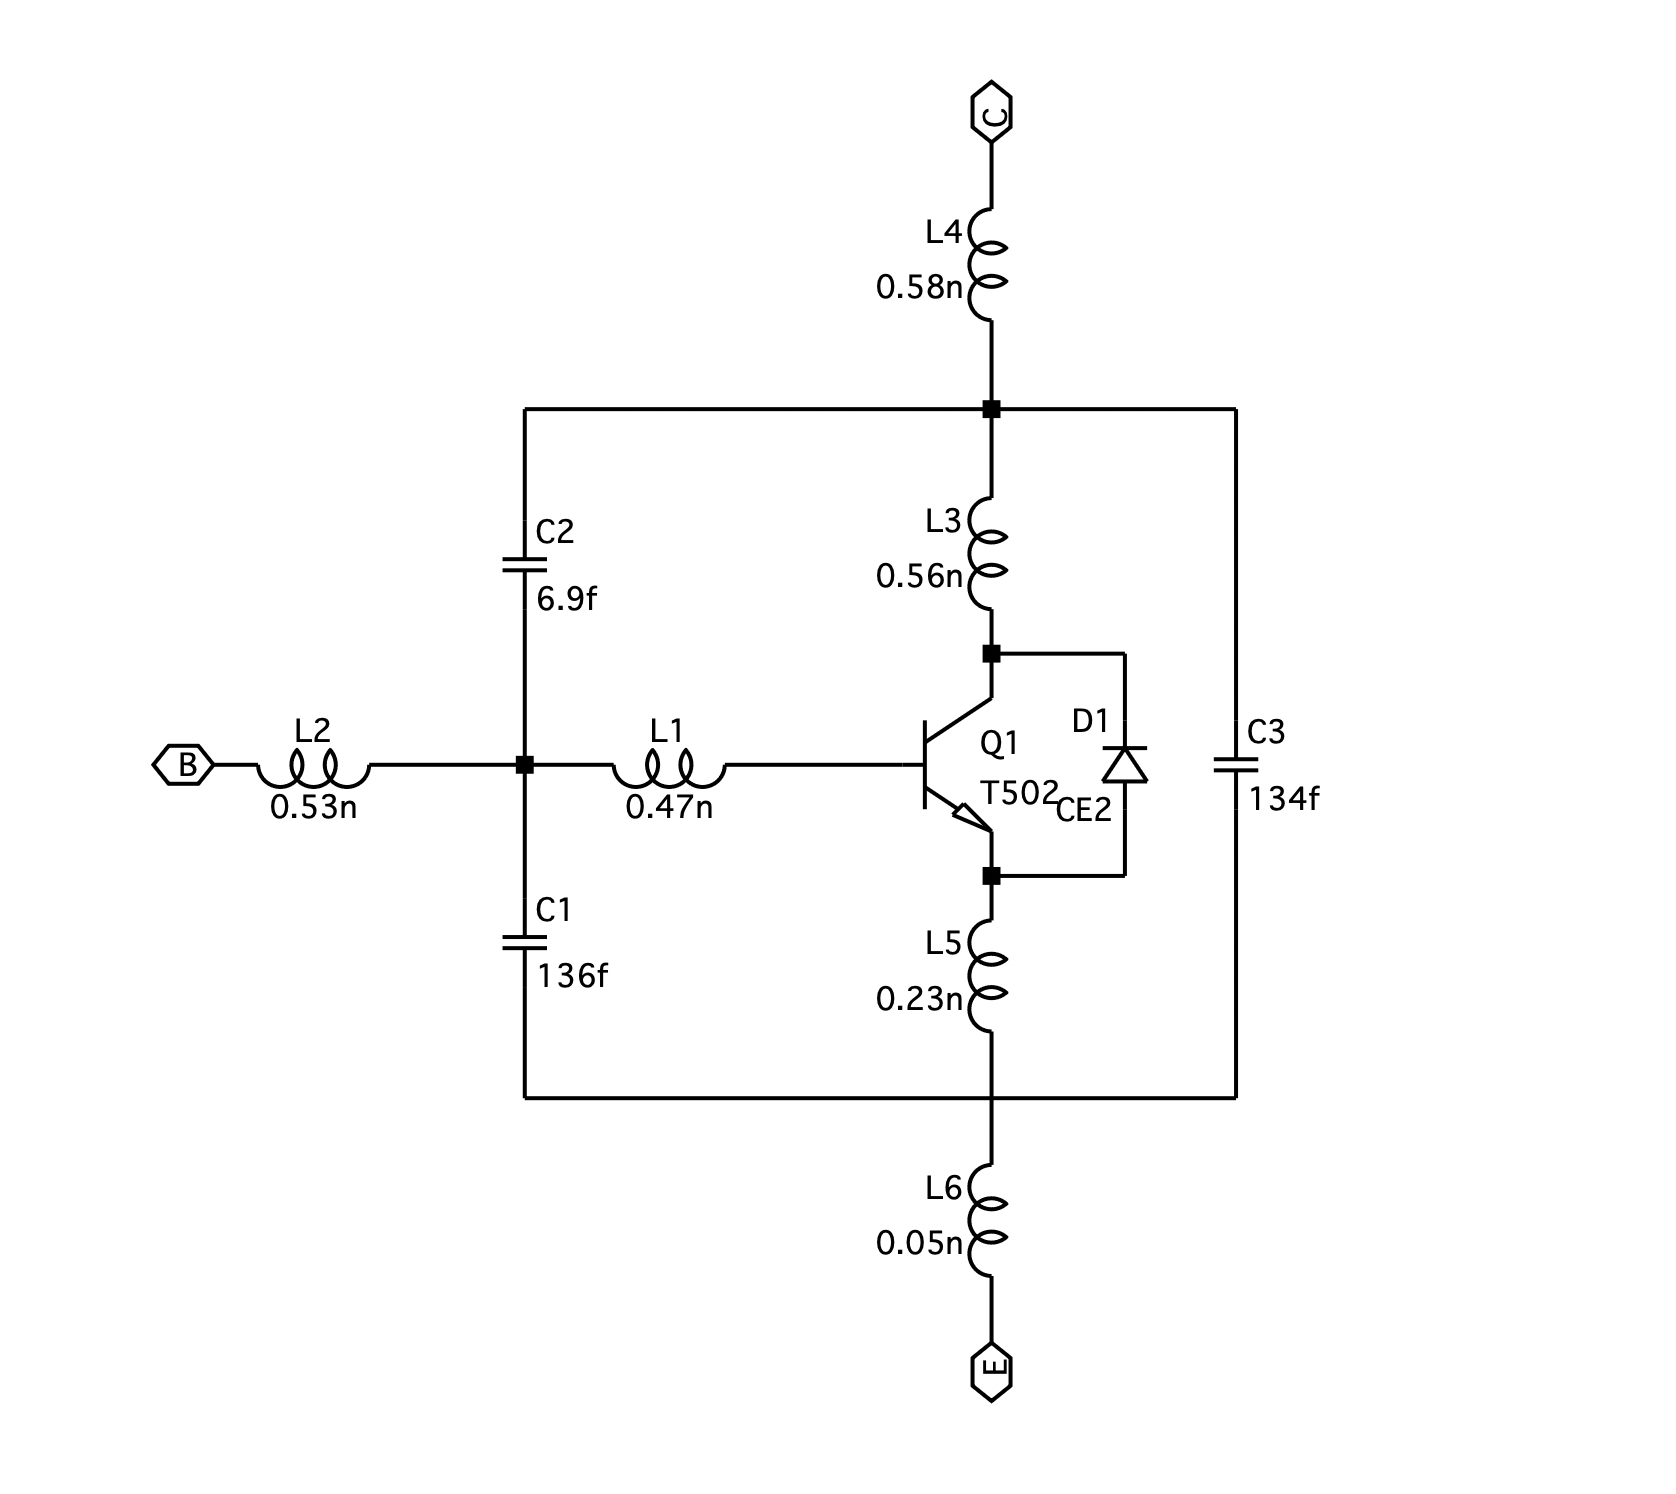
\includegraphics[width=0.6\textwidth]{Images/TransistorReal.png}
    \caption{Transistor with packaging effects.}
    \label{fig:TransistorReal}
\end{figure}

In a transistor simulation that can be close to the real one, the biasing circuit is essential to ensure that the transistor operates in the correct region. The biasing circuit was designed to provide the necessary DC voltage and current required in the initial parameters, so it can operate properly. The biasing circuit can be seen in Figure \ref{fig:SIMBiasCircuit}.

\begin{figure}[H]
    \centering
    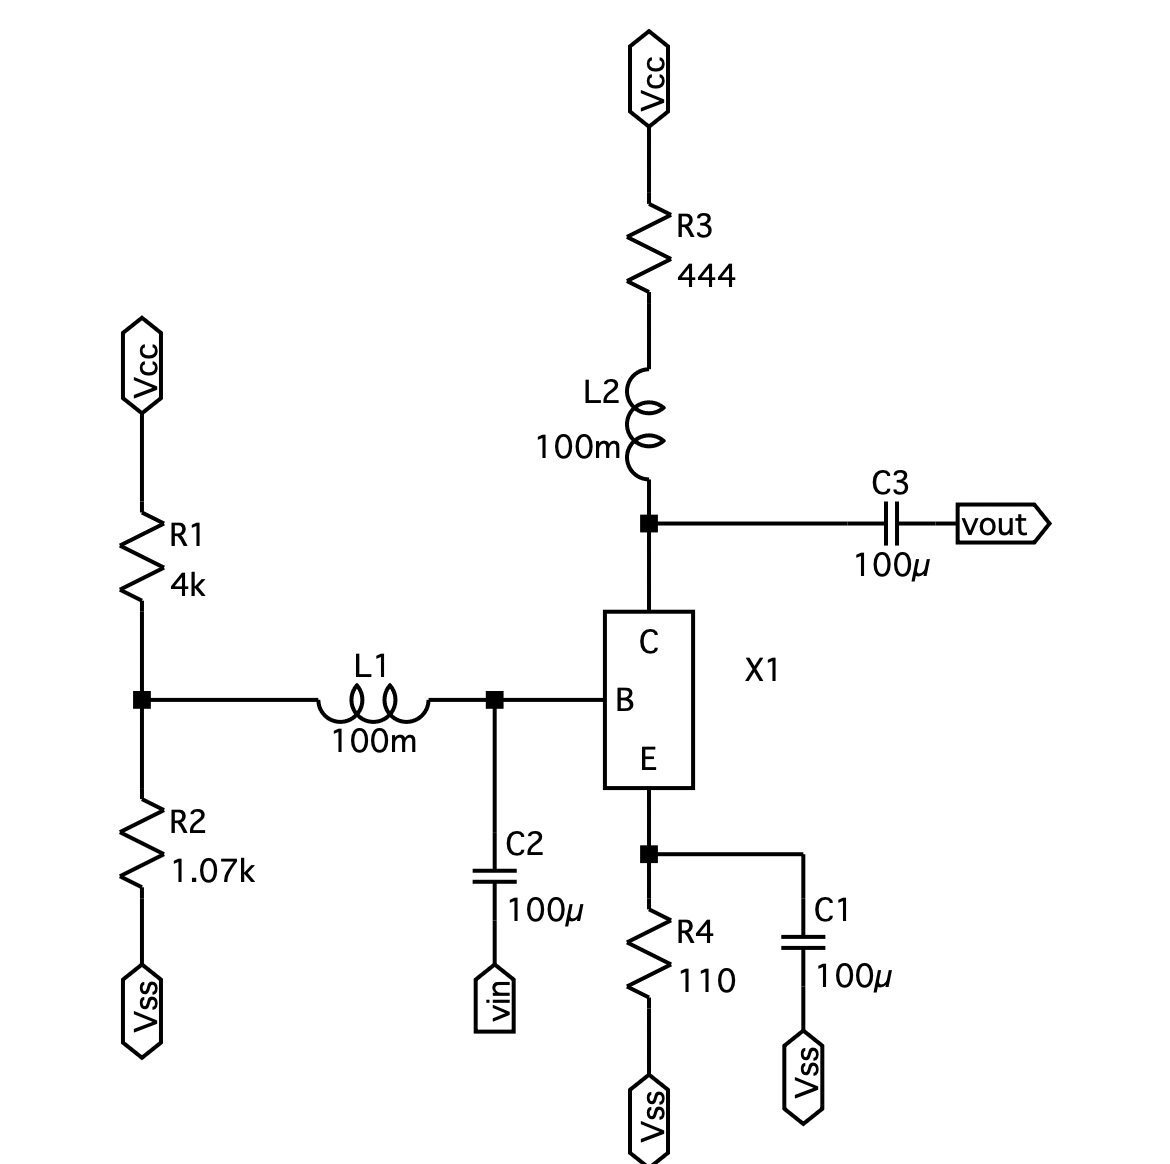
\includegraphics[width=0.5\textwidth]{Images/SIMBiasCircuit.png}
    \caption{Biasing circuit simulated.}
    \label{fig:SIMBiasCircuit}
\end{figure}

The operating point of the circuit was simulated using LTSpice, where the DC analysis was performed to obtain the biasing parameters. The goal is to ensure that the transistor operates in the active region, which is essential for amplification. The parameters to be obtained are the DC voltage at the collector ($V_{CE}$), the DC voltage at the base ($V_{BE}$), and the DC current at the collector ($I_{C}$).

The results of the operation point simulation is shown in Figure \ref{fig:SIMBias}.

\begin{figure}[H]
    \centering
    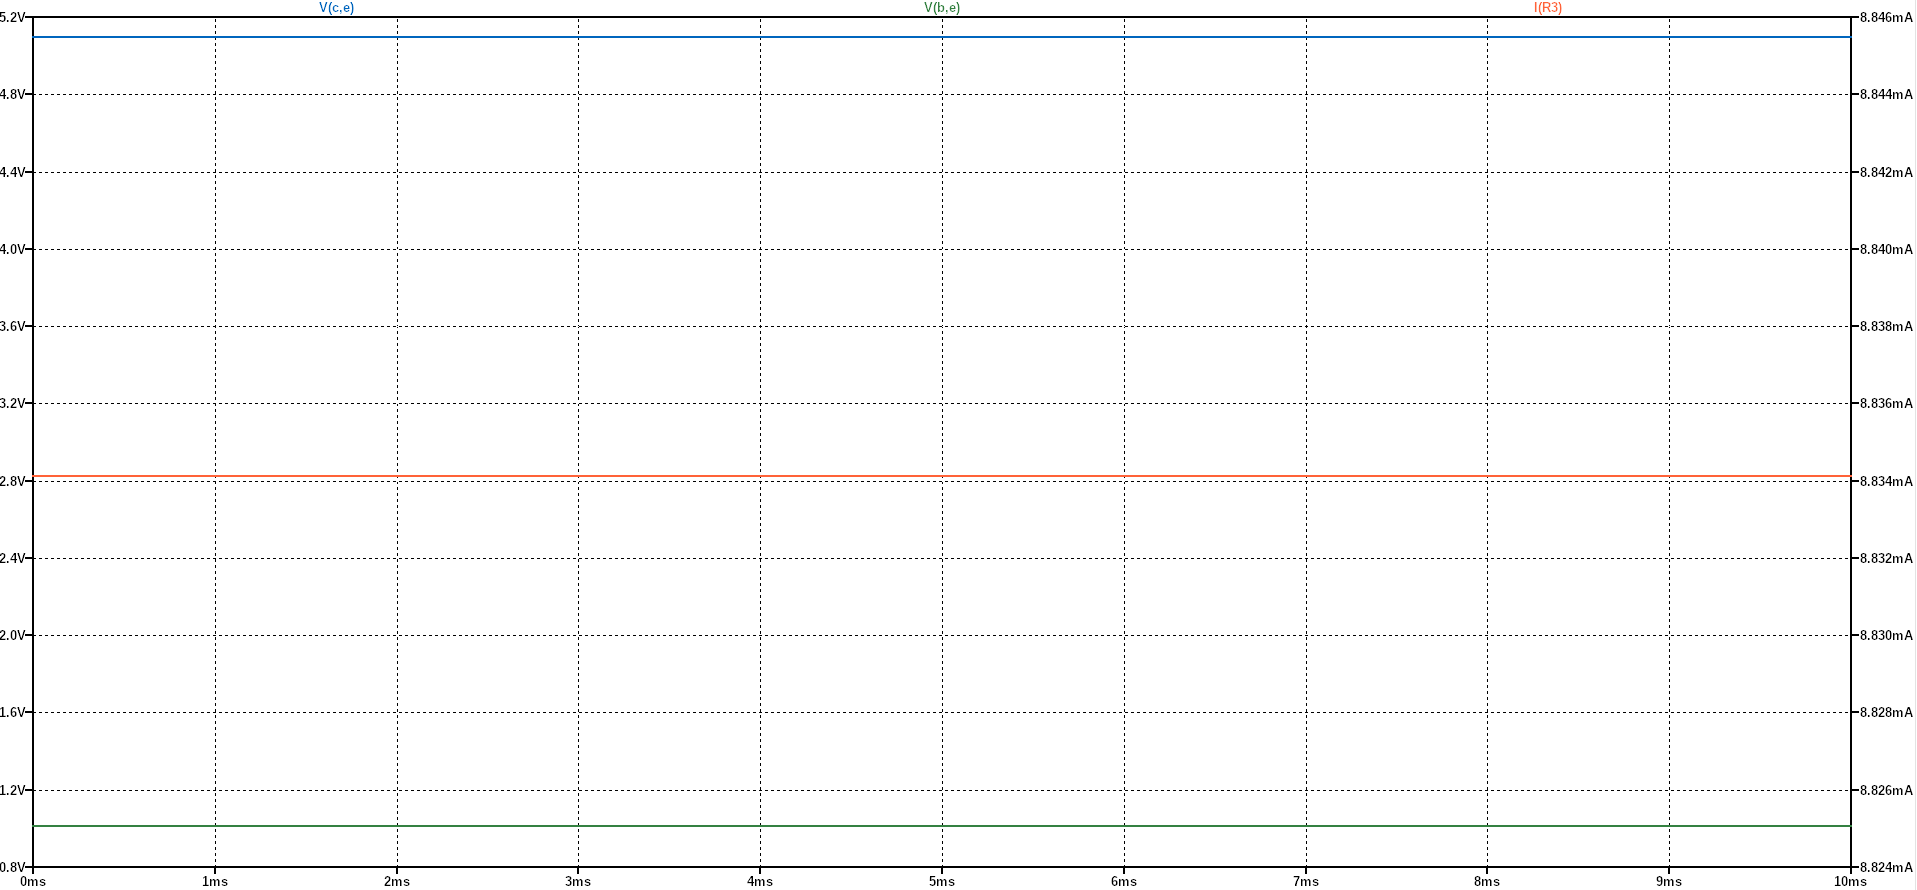
\includegraphics[width=1\textwidth]{Images/SIMBias.png}
    \caption{Result of the operating point simulation.}
    \label{fig:SIMBias}
\end{figure}

In table \ref{tab:BiasingParameters} the results of the biasing circuit are summarized.

\begin{table}[H]
    \centering
    \caption{Biasing circuit parameters.}
    \begin{tabularx}{\textwidth}{>{\centering\arraybackslash}X >{\centering\arraybackslash}X}
        \toprule
        \textbf{Parameter} & \textbf{Value} \\
        \midrule
        $V_{CE}$ & 5.094 V \\
        \midrule
        $V_{BE}$ & 1.012 V \\
        \midrule
        $I_{C}$ & 8.83 \si{\milli \ampere} \\
        \bottomrule
    \end{tabularx}
    \label{tab:BiasingParameters}
\end{table}

The results obtain are within the required parameters for the biasing circuit designed in the previous section. With the transistor biasing validated was possible to proceed with the simulations for the matching networks.

At the same time, the same circuit was implemented in Cadence, to ensure greater reliability of the results obtained. The schematic implementation in Cadence can be seen in Figure \ref{fig:CadenceBiasCircuit}.

\begin{figure}[H]
    \centering
    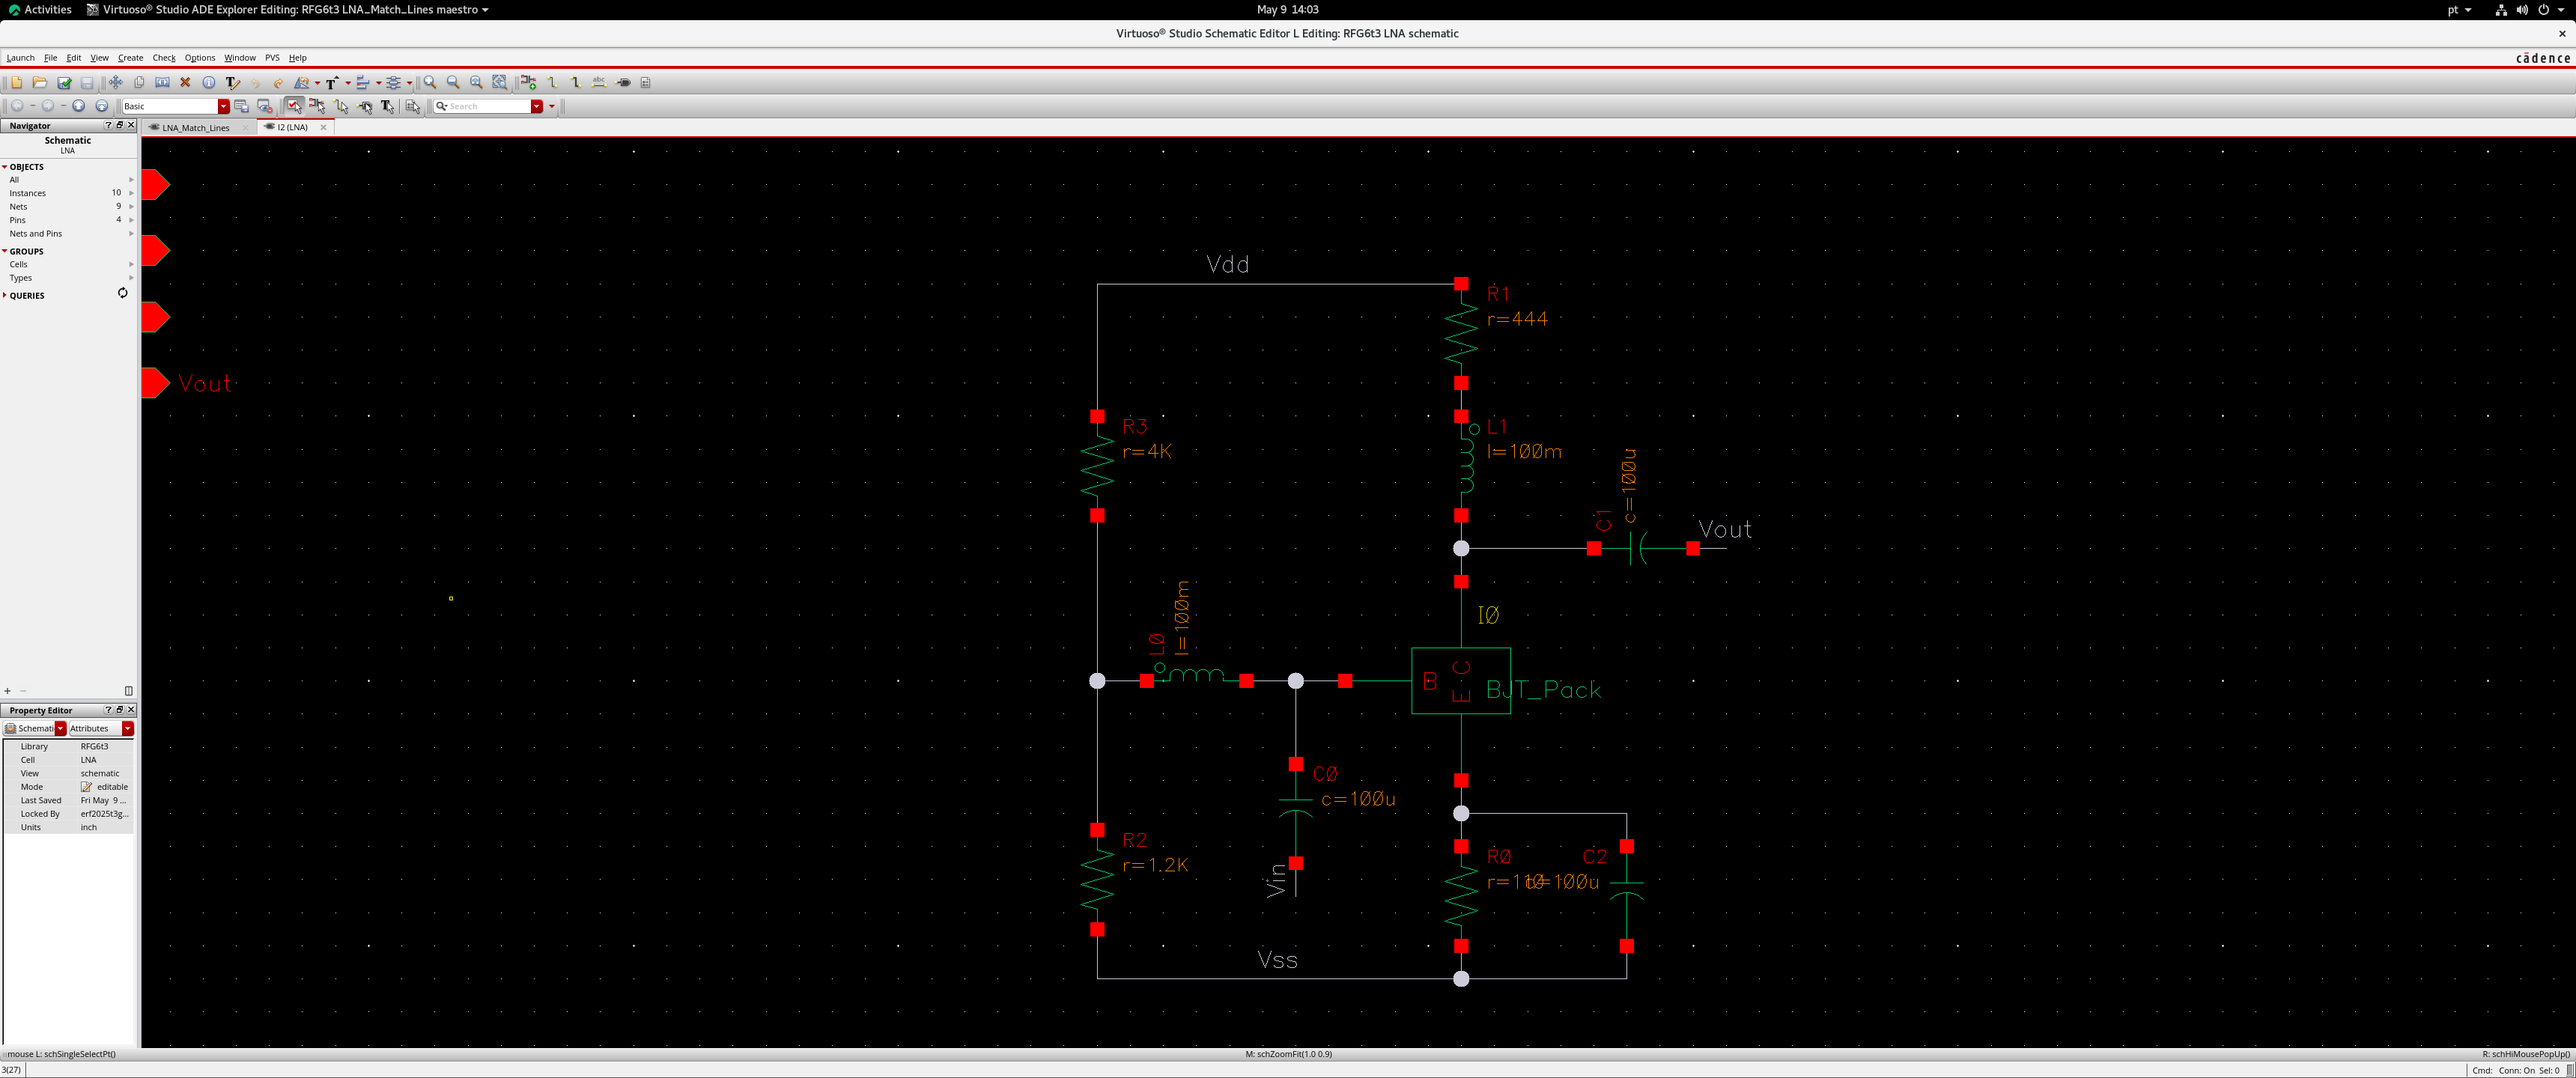
\includegraphics[width=1\textwidth]{Images/CadenceBiascircuit.png}
    \caption{Biasing circuit simulated in Cadence}
    \label{fig:CadenceBiasCircuit}
\end{figure}

\subsection{Simulation without matching networks}

As mentioned before, the first step in designing a matching network of an LNA is to know the S-parameters of the amplifier circuit for the range of frequencies, so, switching to an AC analysis of the LNA circuit, and adding both the source and the load ($50 \si{\ohm}$), the schematic of the simulated circuit in LTSpice is shown in Figure \ref{fig:SIMS-paramCircuit}.

\begin{figure}[H]
    \centering
    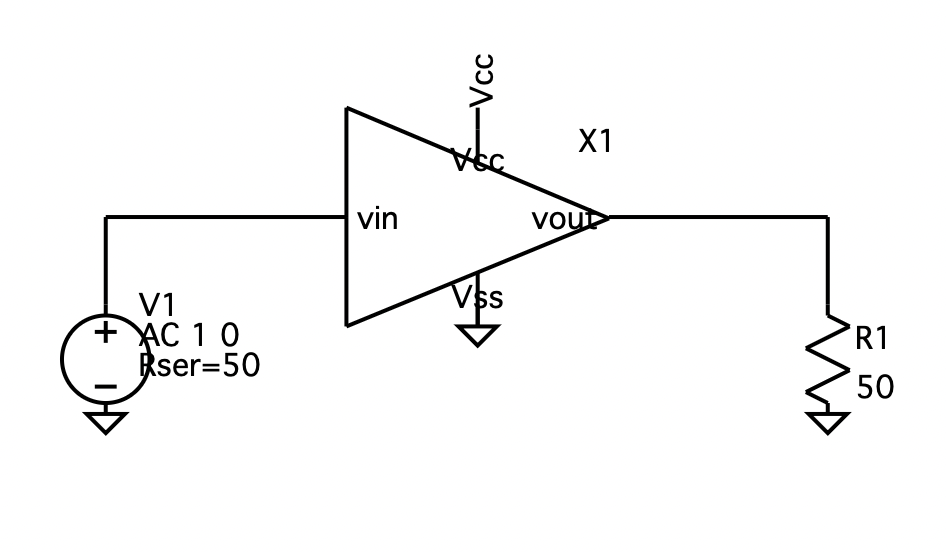
\includegraphics[width=0.5\textwidth]{Images/S-paramCircuit.png}
    \caption{Circuit for the S-parameters}
    \label{fig:SIMS-paramCircuit}
\end{figure}

The resulting S-parameters obtain in LTSpice were extracted to a s2p file and further processed in a Python script \ref{appendix:python_script}, the resultant s-parameters without matching networks in LTSpice can be seen in Figure \ref{fig:SimS-param}.

\begin{figure}[H]
    \centering
    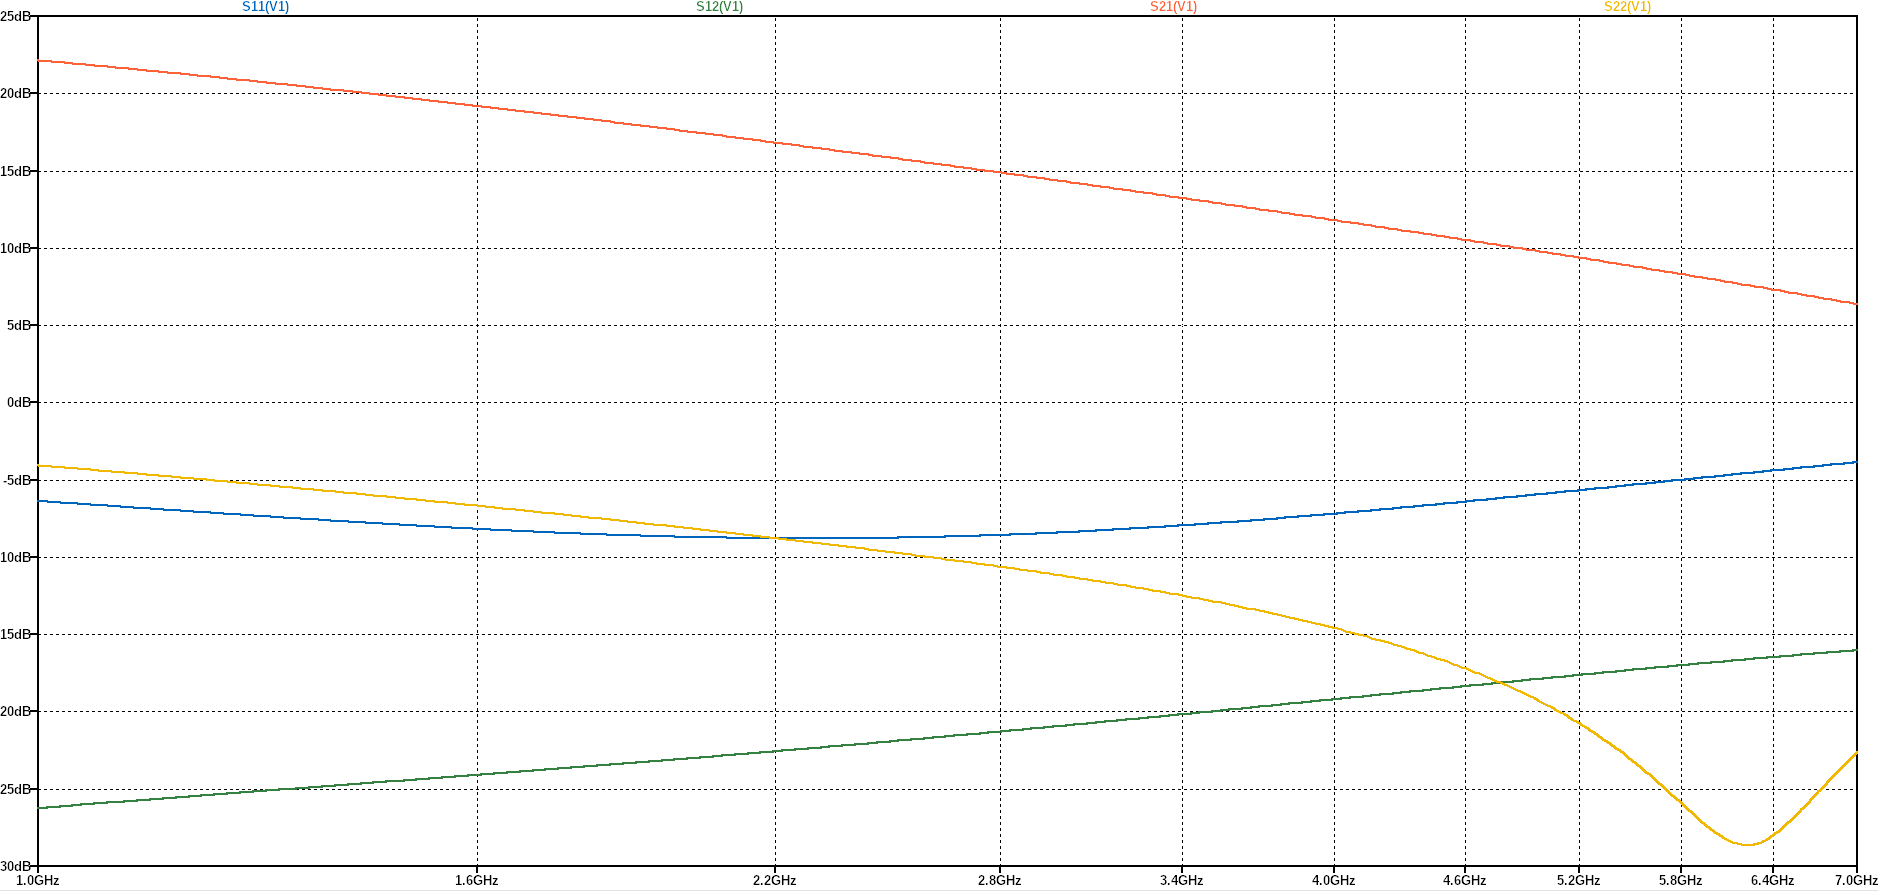
\includegraphics[width=1\textwidth]{Images/SIM-s-param-nomatch.png}
    \caption{S-parameters for the LNA circuit}
    \label{fig:SimS-param}
\end{figure}

The same simulation was done in Cadence, and the results can be seen in Figure \ref{fig:CadenceS-param}.
\begin{figure}[H]
    \centering
    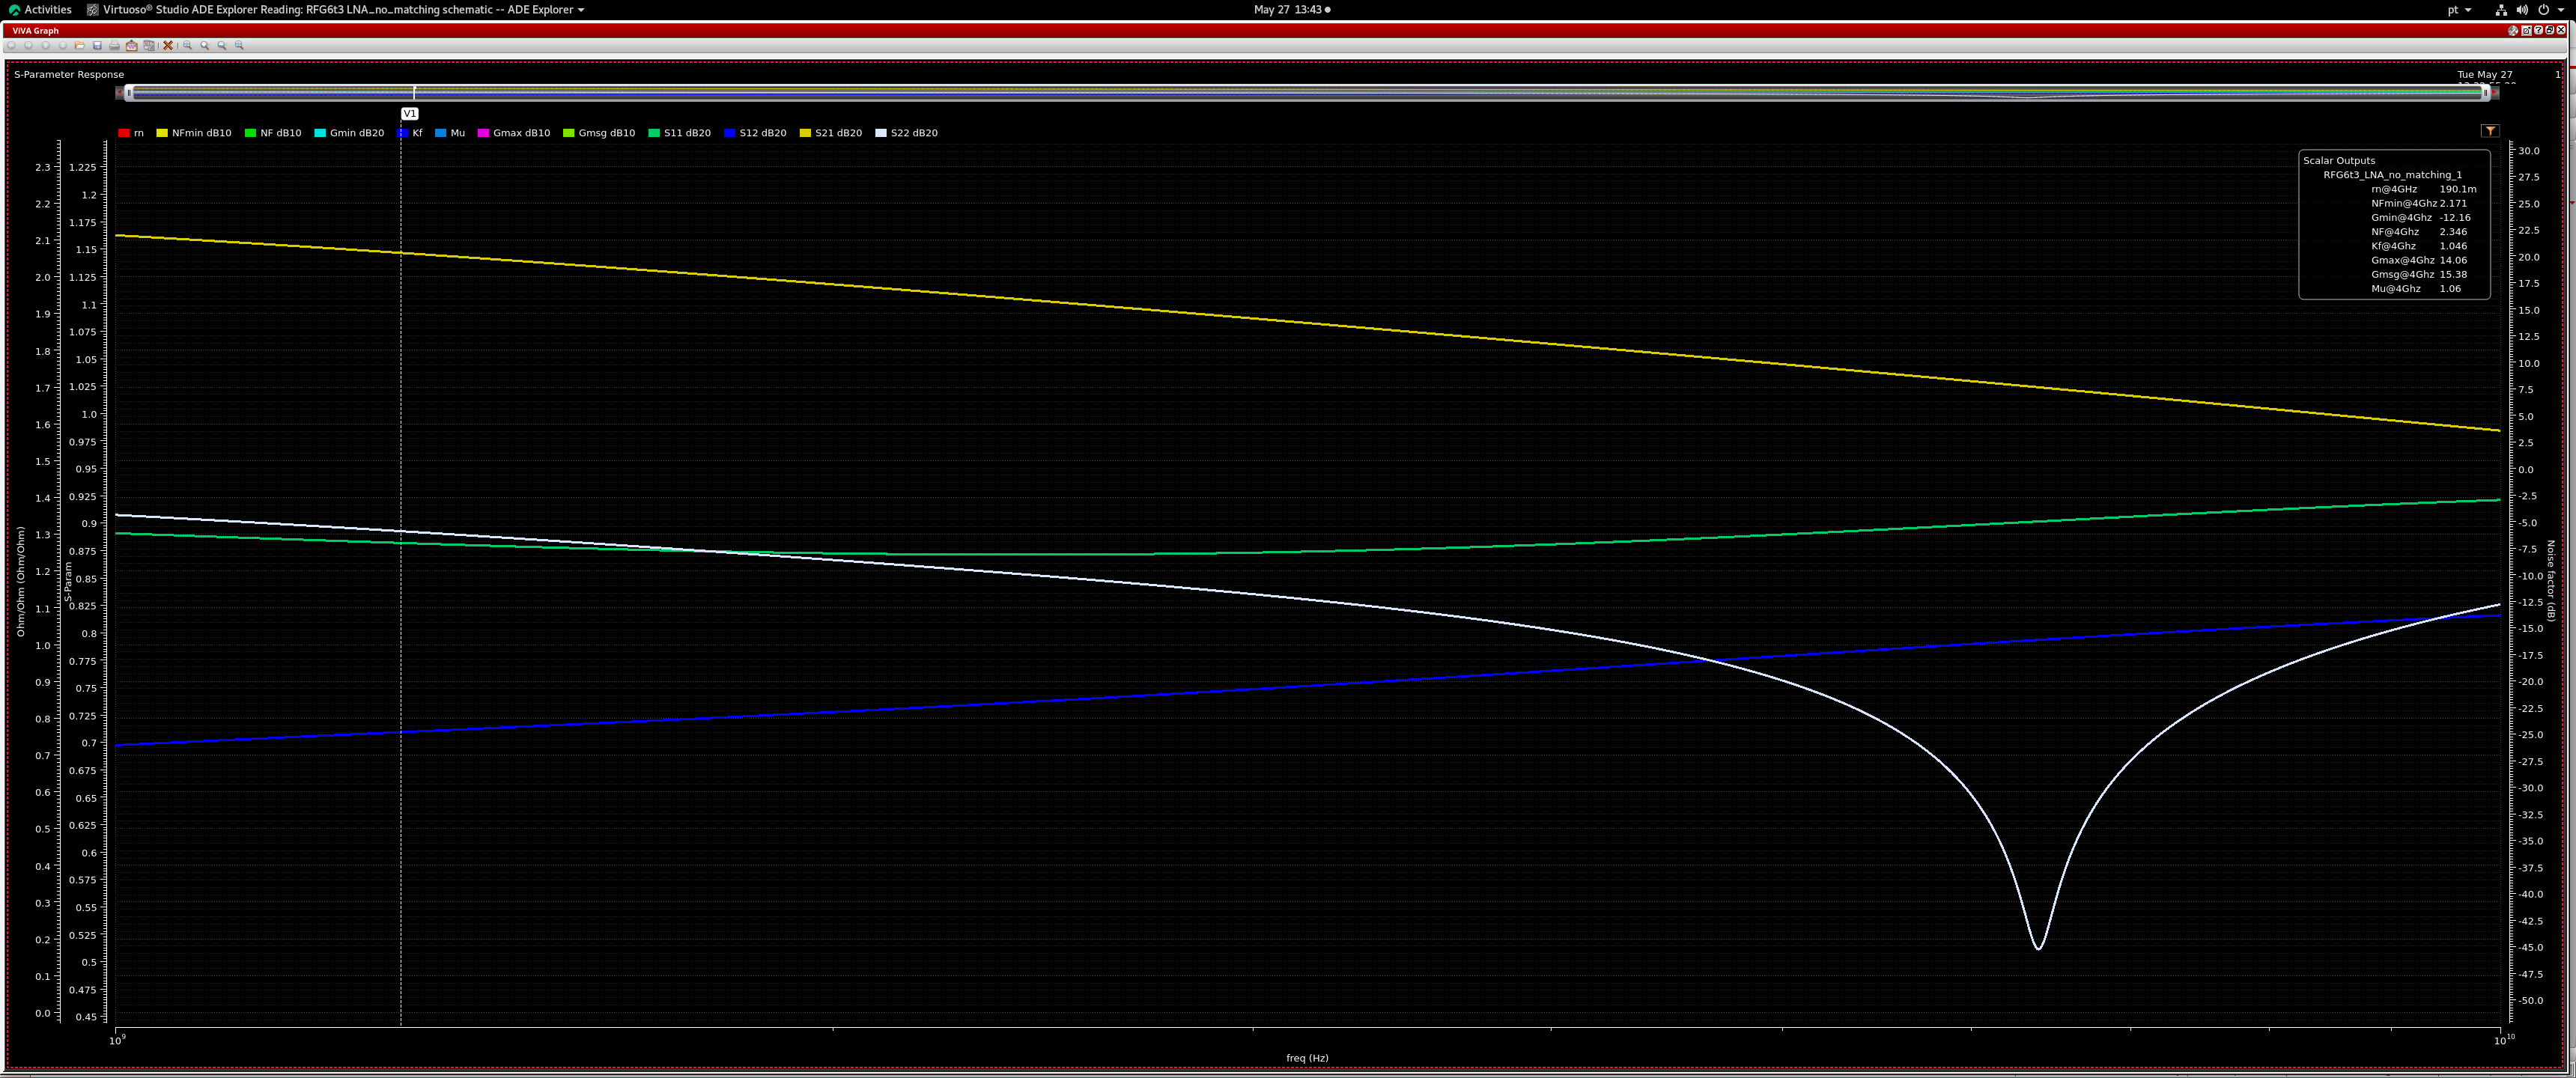
\includegraphics[width=1\textwidth]{Images/cad-s-param-no-match.png}
    \caption{S-parameters for the LNA circuit in Cadence.}
    \label{fig:CadenceS-param}
\end{figure}

\subsection{Simulation for Maximum Gain Adaptation}

After assuming a working frequency of $4 GHz$ at the previous section, the resulting matching networks for maximum gain were simulated, first in LTSpice and then in Cadence, in order to validate the results obtained.

\subsubsection{Matching networks using Lumped circuit elements}

The matching networks for input and output depicted in Figure \ref{fig:zs-LC-matching} were used to perform the simulation and validate the results.

First, the simulation was done in LTSpice and the results can be seen in Figure \ref{fig:SIMLCMatchingCircuit}.
\begin{figure}[H]
    \centering
    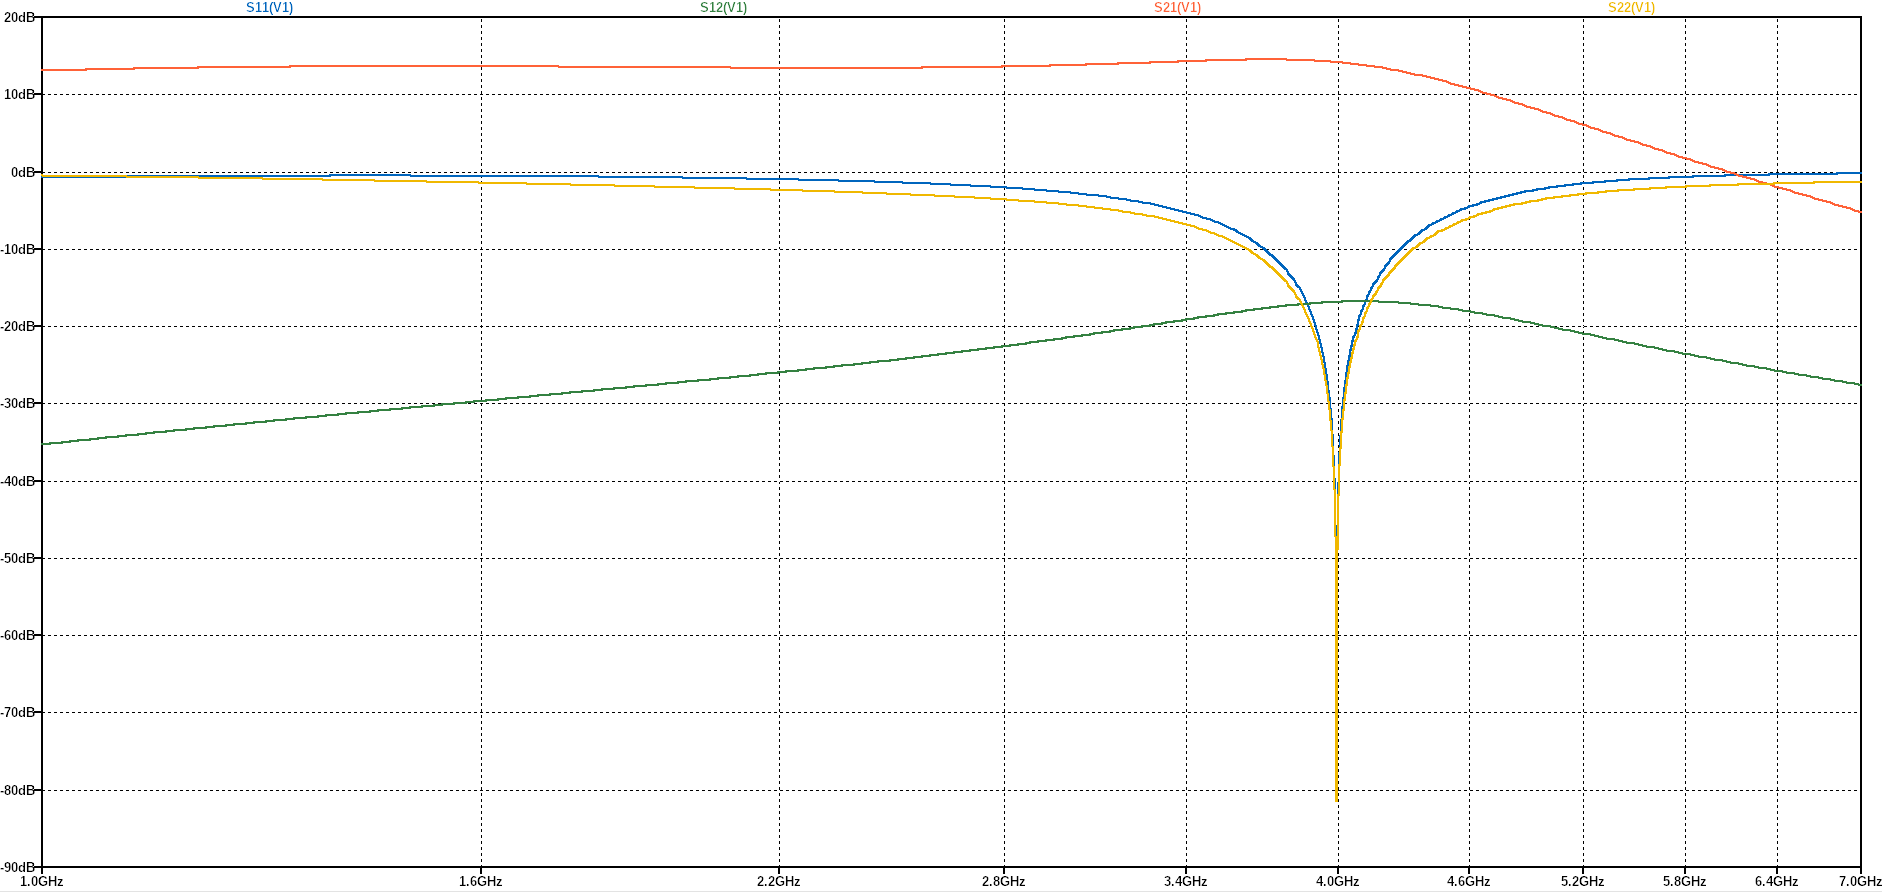
\includegraphics[width=1\textwidth]{Images/LT-LC-gain.png}
    \caption{Matching networks using lumped circuit elements in LTSpice.}
    \label{fig:SIMLCMatchingCircuit}
\end{figure}

After looking at the graphic above, it is possible to conclude that this matching network is working properly, since there is a sharp drop in both $S11$ and $S22$ at the desired frequency of $4GHz$ as well as a high point in the $S21$ curve that is the maximum gain of the circuit, which is around $14 dB$ as expected.

For more accurate results, the same circuit was simulated in Cadence, and the schematic can be seen in Figure \ref{fig:CadenceLCMatchingCircuit}.
\begin{figure}[H]
    \centering
    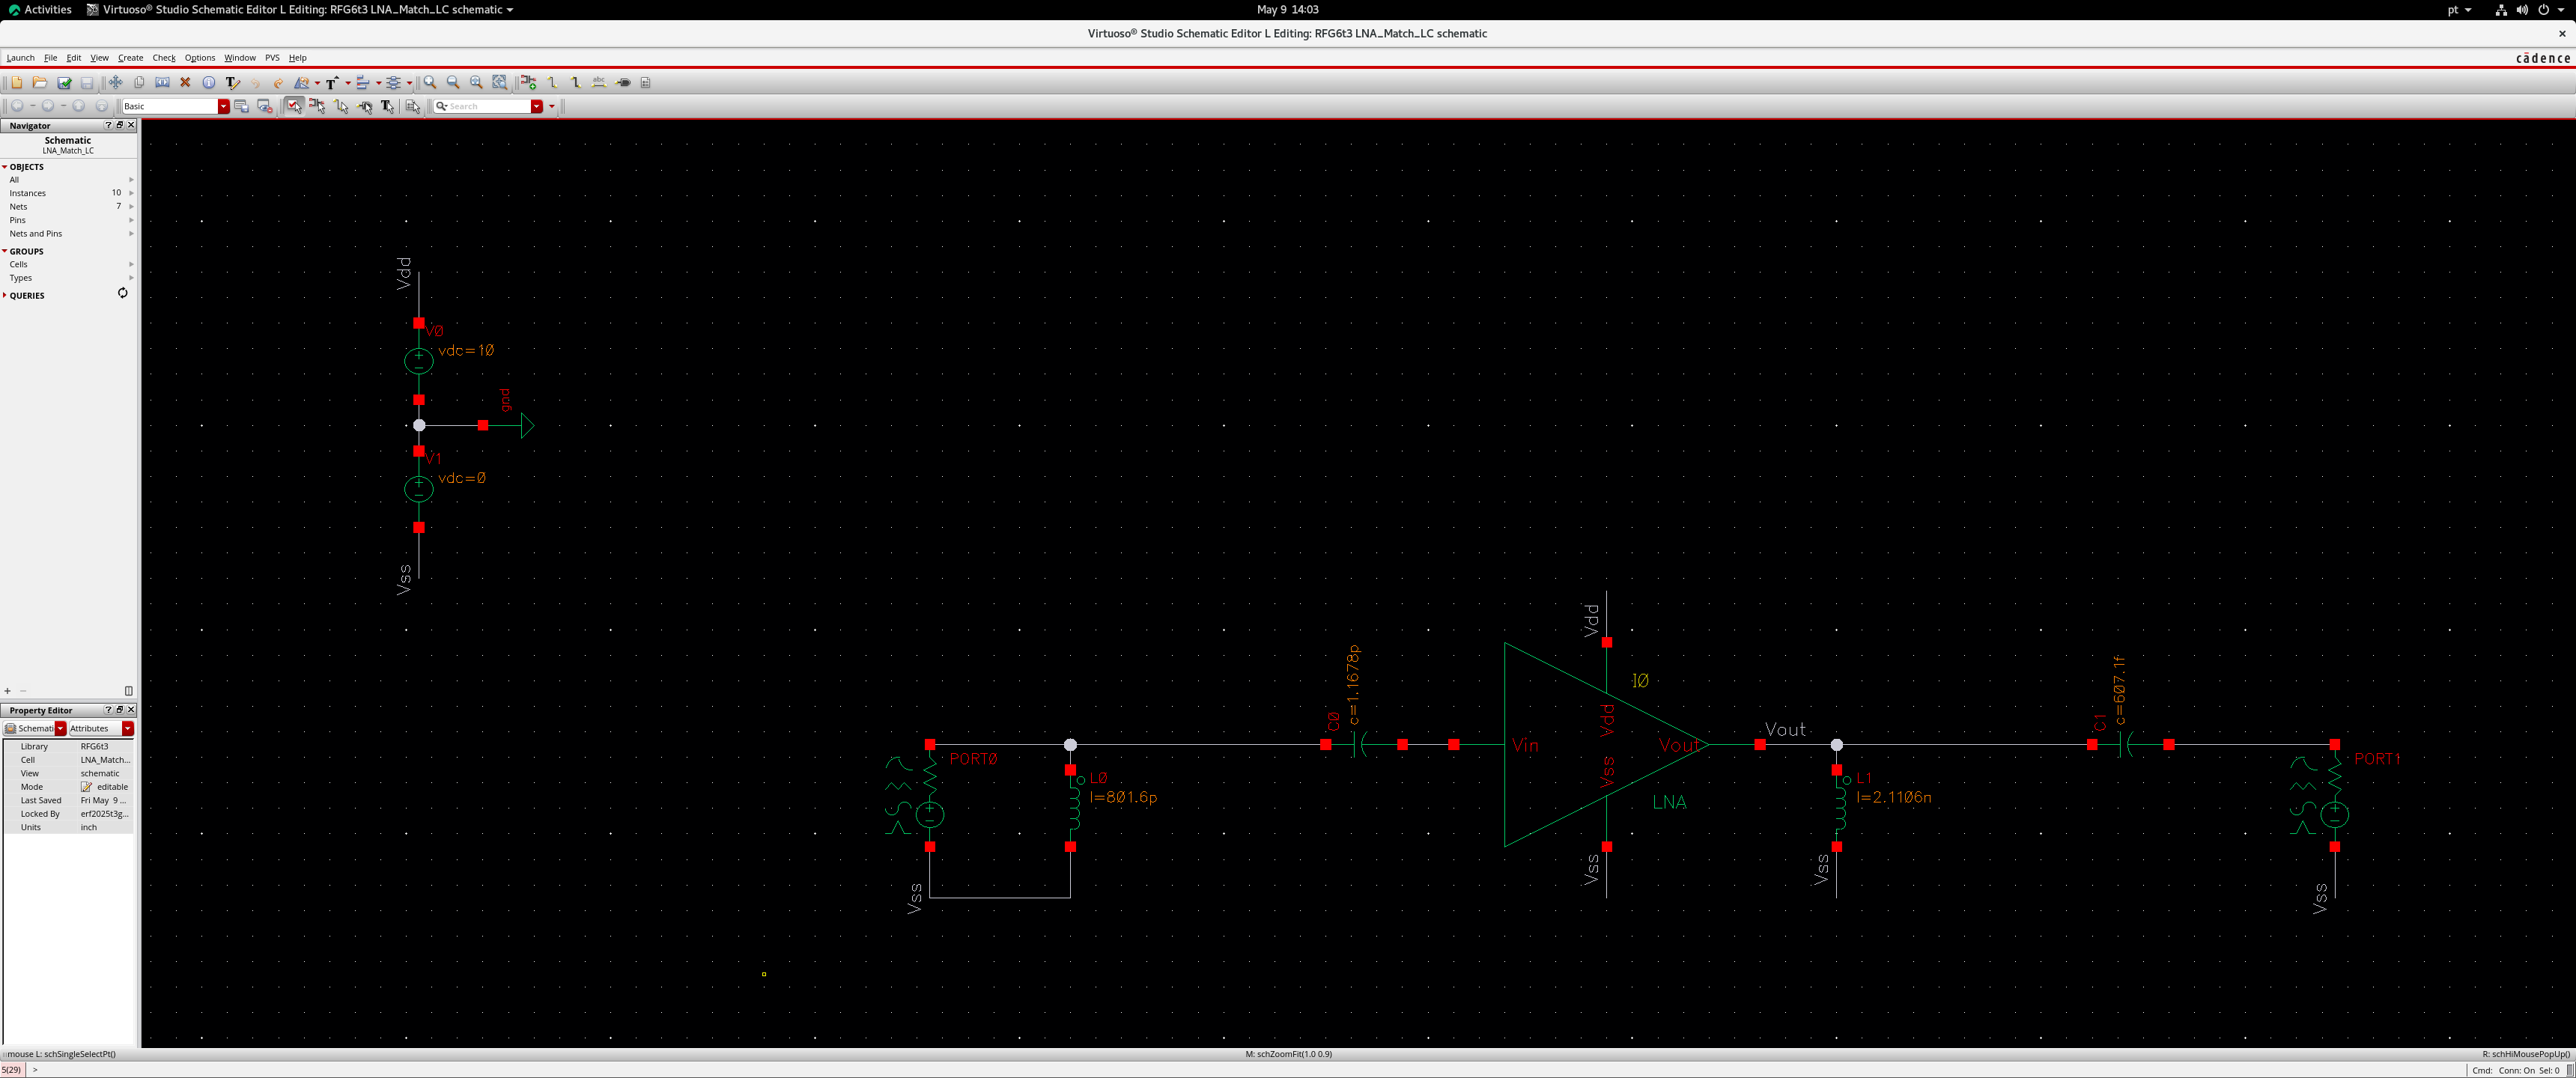
\includegraphics[width=1\textwidth]{Images/CadenceLCcircuit.png}
    \caption{Matching networks using lumped circuit elements in Cadence.}
    \label{fig:CadenceLCMatchingCircuit}
\end{figure}

The graphical results of the simulation in Cadence can be seen in Figure \ref{fig:CadenceLC}.
\begin{figure}[H]
    \centering
    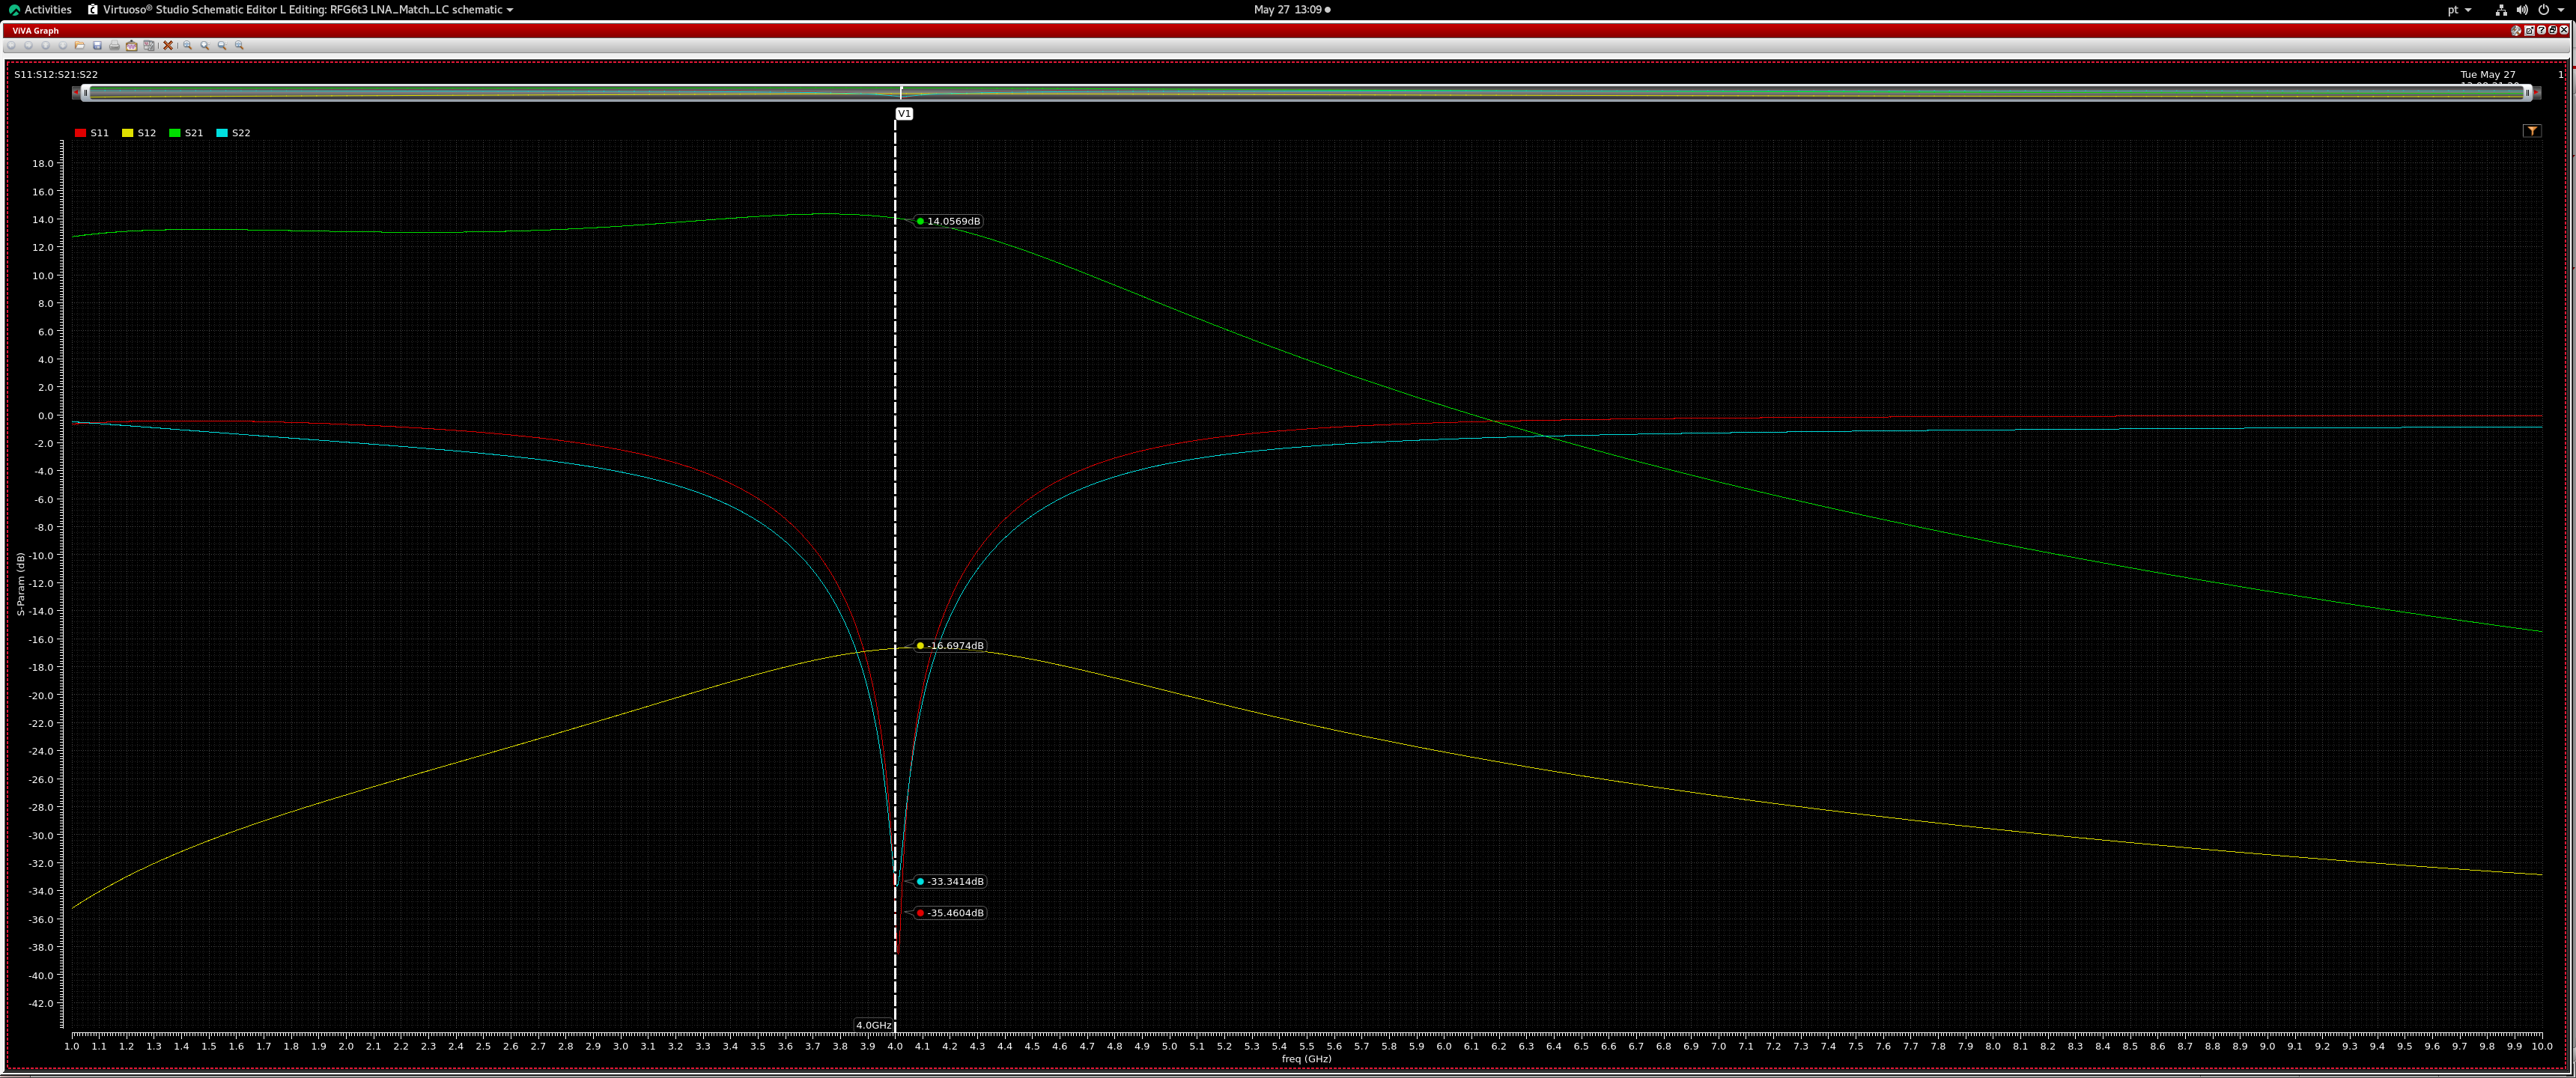
\includegraphics[width=1\textwidth]{Images/CAD-LC_matching.png}
    \caption{S-parameters for the matching networks using lumped circuit elements in Cadence.}
    \label{fig:CadenceLC}
\end{figure}

In table \ref{tab:LCMatchingParameters} the results of the matching networks using lumped circuit elements are summarized.

\begin{table}[H]
    \centering
    \caption{Matching network results using lumped circuit elements in Cadence.}
    \begin{tabularx}{\textwidth}{>{\centering\arraybackslash}X >{\centering\arraybackslash}X}
        \toprule
        \textbf{Parameter} & \textbf{Value} \\
        \midrule
        LTSpice $S21$  & $14.18 \si{\decibel}$ \\
        \midrule
        Cadence $S21$ & $14.06 \si{\decibel}$ \\
        \bottomrule
    \end{tabularx}
    \label{tab:LCMatchingParameters}
\end{table}

Observing the results, it is possible to conclude that the matching networks using lumped circuit elements are working properly, since the $S21$ parameter is around $14 dB$ in both LTSpice and Cadence, which is close to the expected value of $14,17 dB$ calculated in the previous section.

\subsubsection{Matching networks using transmission lines and stubs}

The matching networks for input and output depicted in Figure \ref{fig:MatchingCircuit-line} were used to perform the simulation and validate the results.

First, the simulation was done in LTSpice and the results can be seen in Figure \ref{fig:LT-LSMatchingCircuit}.
\begin{figure}[H]
    \centering
    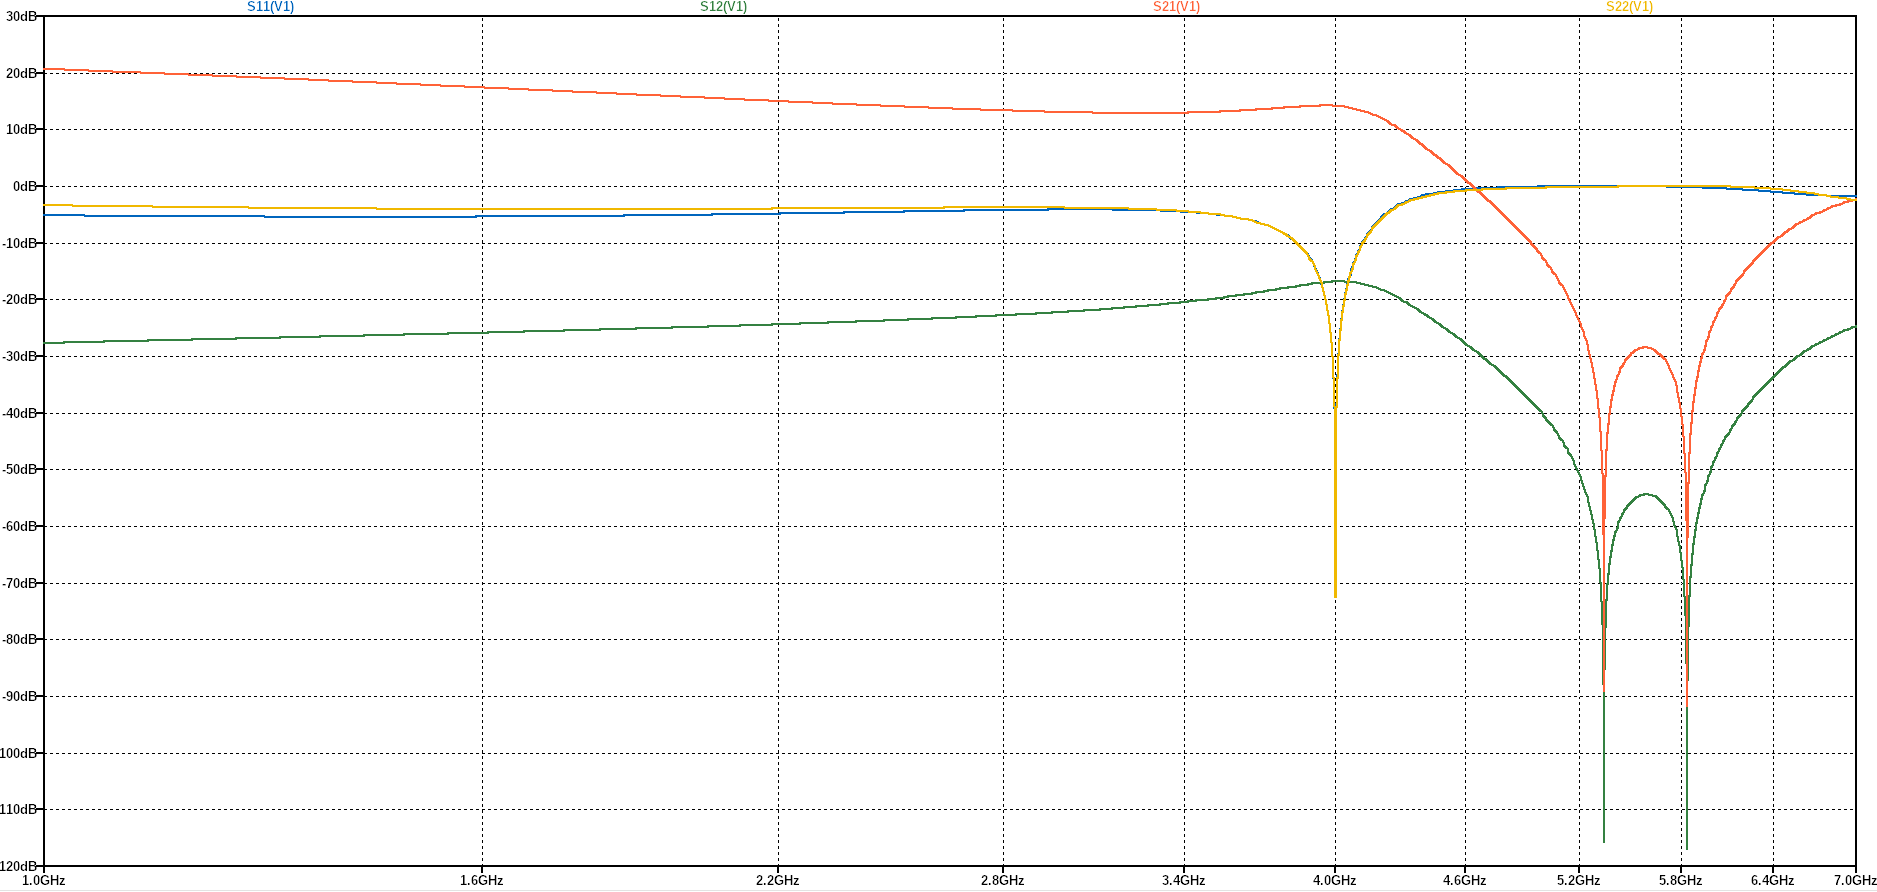
\includegraphics[width=1\textwidth]{Images/LT-LS-gain.png}
    \caption{Matching networks using transmission lines and stubs in LTSpice.}
    \label{fig:LT-LSMatchingCircuit}
\end{figure}

In cadence, the circuit for using transmission lines and stubs is depicted in Figure \ref{fig:CAD-LScircuit}.
\begin{figure}[H]
    \centering
    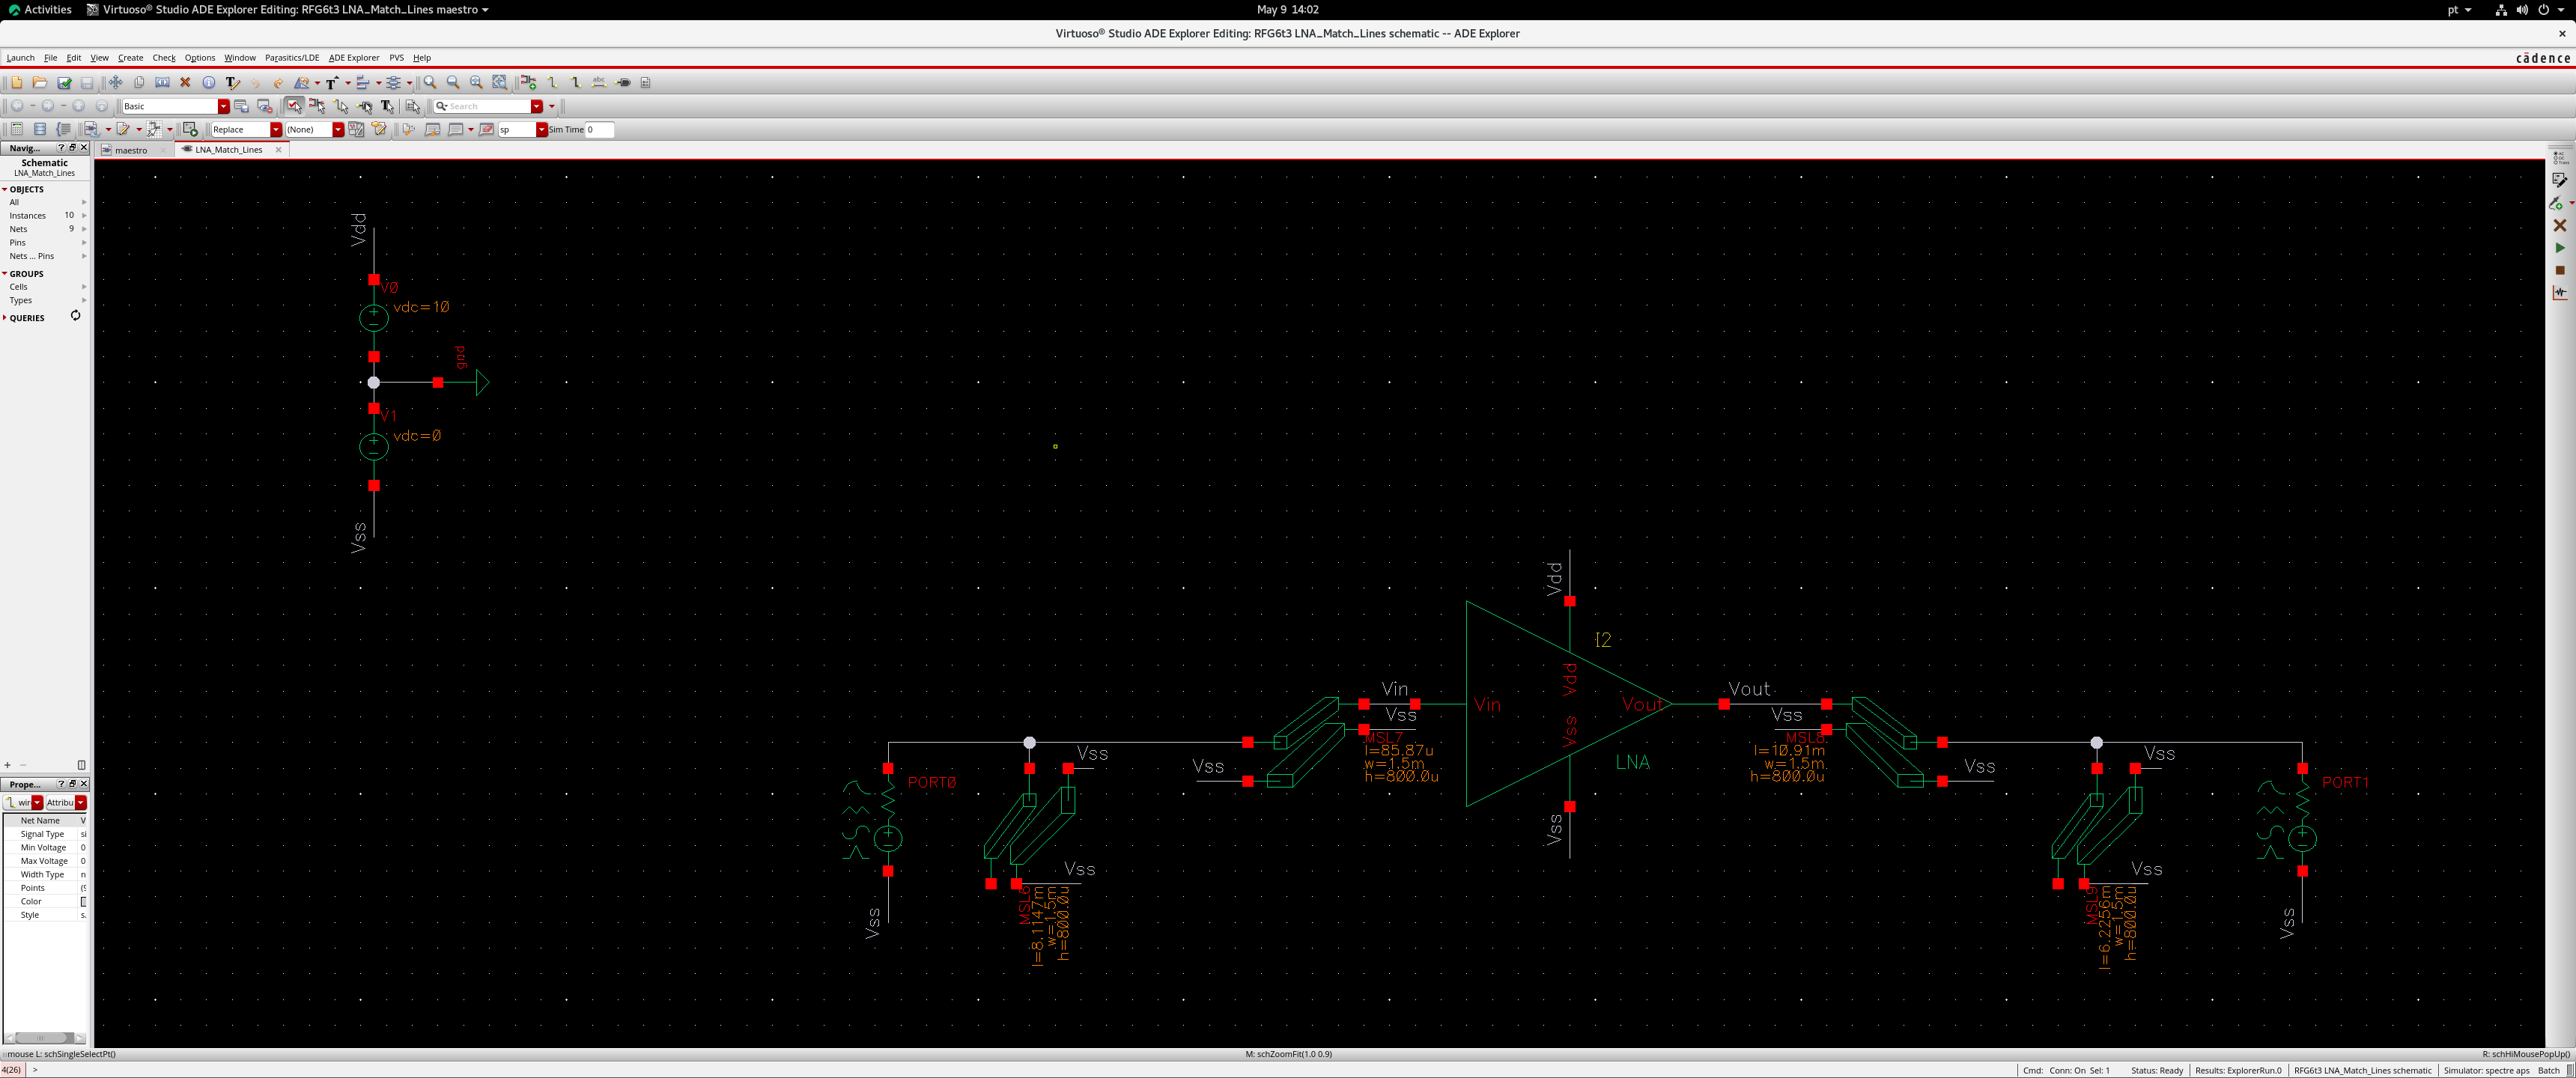
\includegraphics[width=1\textwidth]{Images/CadenceLScircuit.png}
    \caption{Matching networks using transmission lines and stubs in Cadence.}
    \label{fig:CAD-LScircuit}
\end{figure}

The graphical results of the s-parameters simulation in Cadence can be seen in Figure \ref{fig:SIMLSMatching}.
\begin{figure}[H]
    \centering
    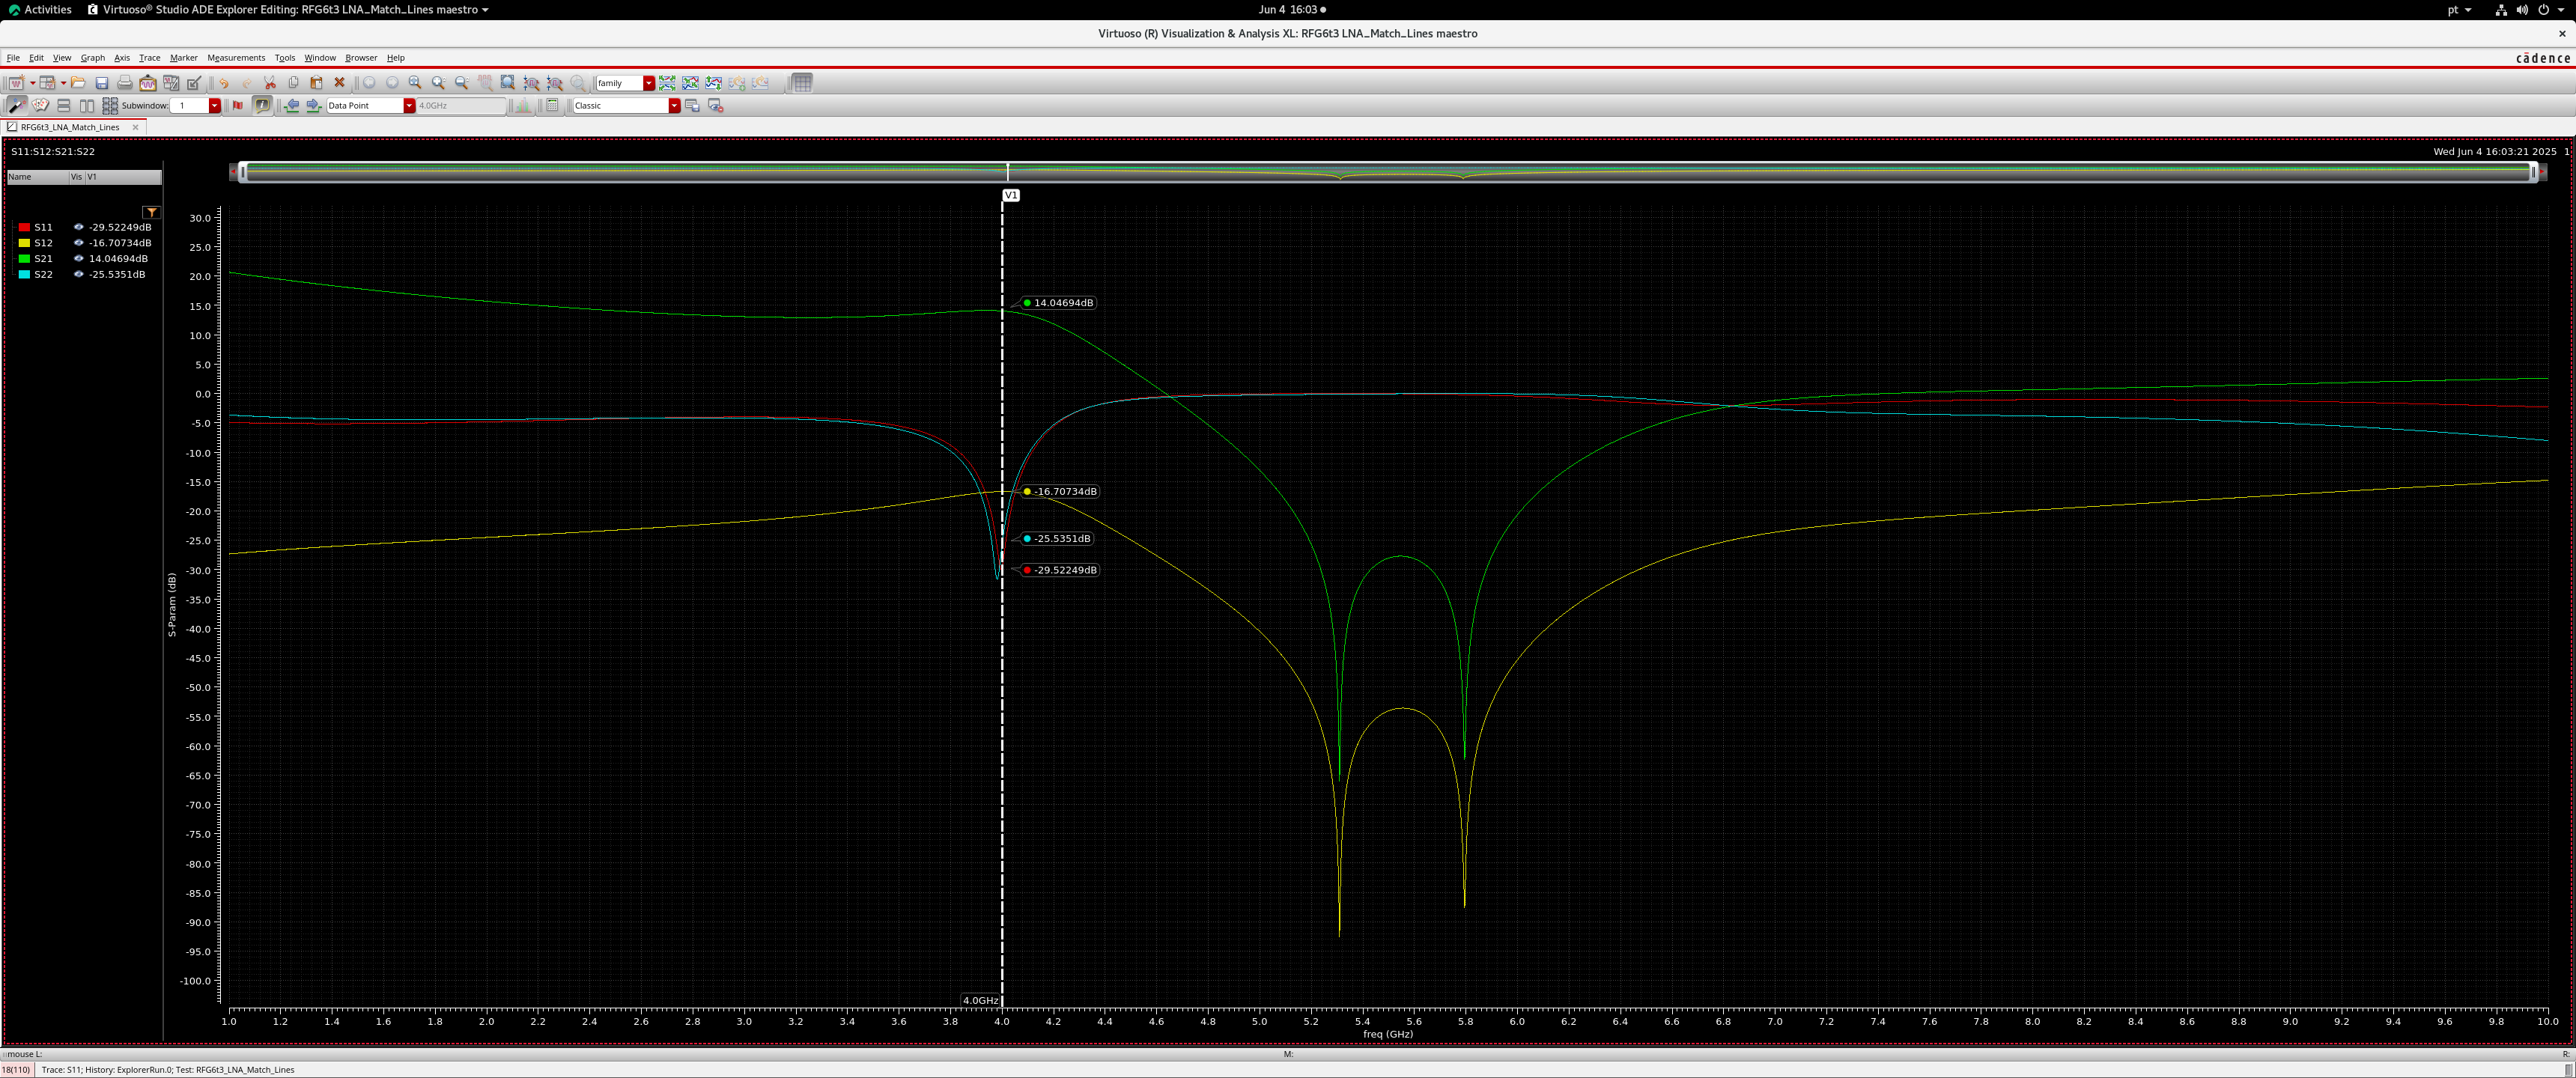
\includegraphics[width=1\textwidth]{Images/CAD-LinesmatchGain.png}
    \caption{S-parameters for the matching networks using transmission lines and stubs in Cadence.}
    \label{fig:SIMLSMatching}
\end{figure}

Similarly to the first matching networks, the drop in both $S11$ and $S22$ can also be seen, as well as the same approximated value of $S21$, so, this matching network using transmission lines and stubs is correctly working. 

The summarized results of the matching networks using transmission lines and stubs can be seen in table \ref{tab:LSMatchingParameters}.
\begin{table}[H]
    \centering
    \caption{Matching network results using transmission lines and stubs in Cadence.}
    \begin{tabularx}{\textwidth}{>{\centering\arraybackslash}X >{\centering\arraybackslash}X}
        \toprule
        \textbf{Parameter} & \textbf{Value} \\
        \midrule
        LTSpice $S21$  & $14.18 \si{\decibel}$ \\
        \midrule
        Cadence $S21$ & $14.05 \si{\decibel}$ \\
        \bottomrule
    \end{tabularx}
    \label{tab:LSMatchingParameters}
\end{table}

\subsection{Simulation for Minimum Noise Adaptation}

In order to adapt the LNA for minimum noise figure, the matching networks were designed to minimize the noise figure at the desired frequency of $4 GHz$, in this section the design matching networks were simulated and validated in Cadence.

\subsubsection{Matching networks using Lumped circuit elements}

The matching networks for input and output depicted in Figure \ref{fig:MatchingCircuit-noise} were used to perform the simulation and validate the results.

The results of the simulation in Cadence can be seen in Figure \ref{fig:CadenceNoiseMatchingCircuit}.
\begin{figure}[H]
    \centering
    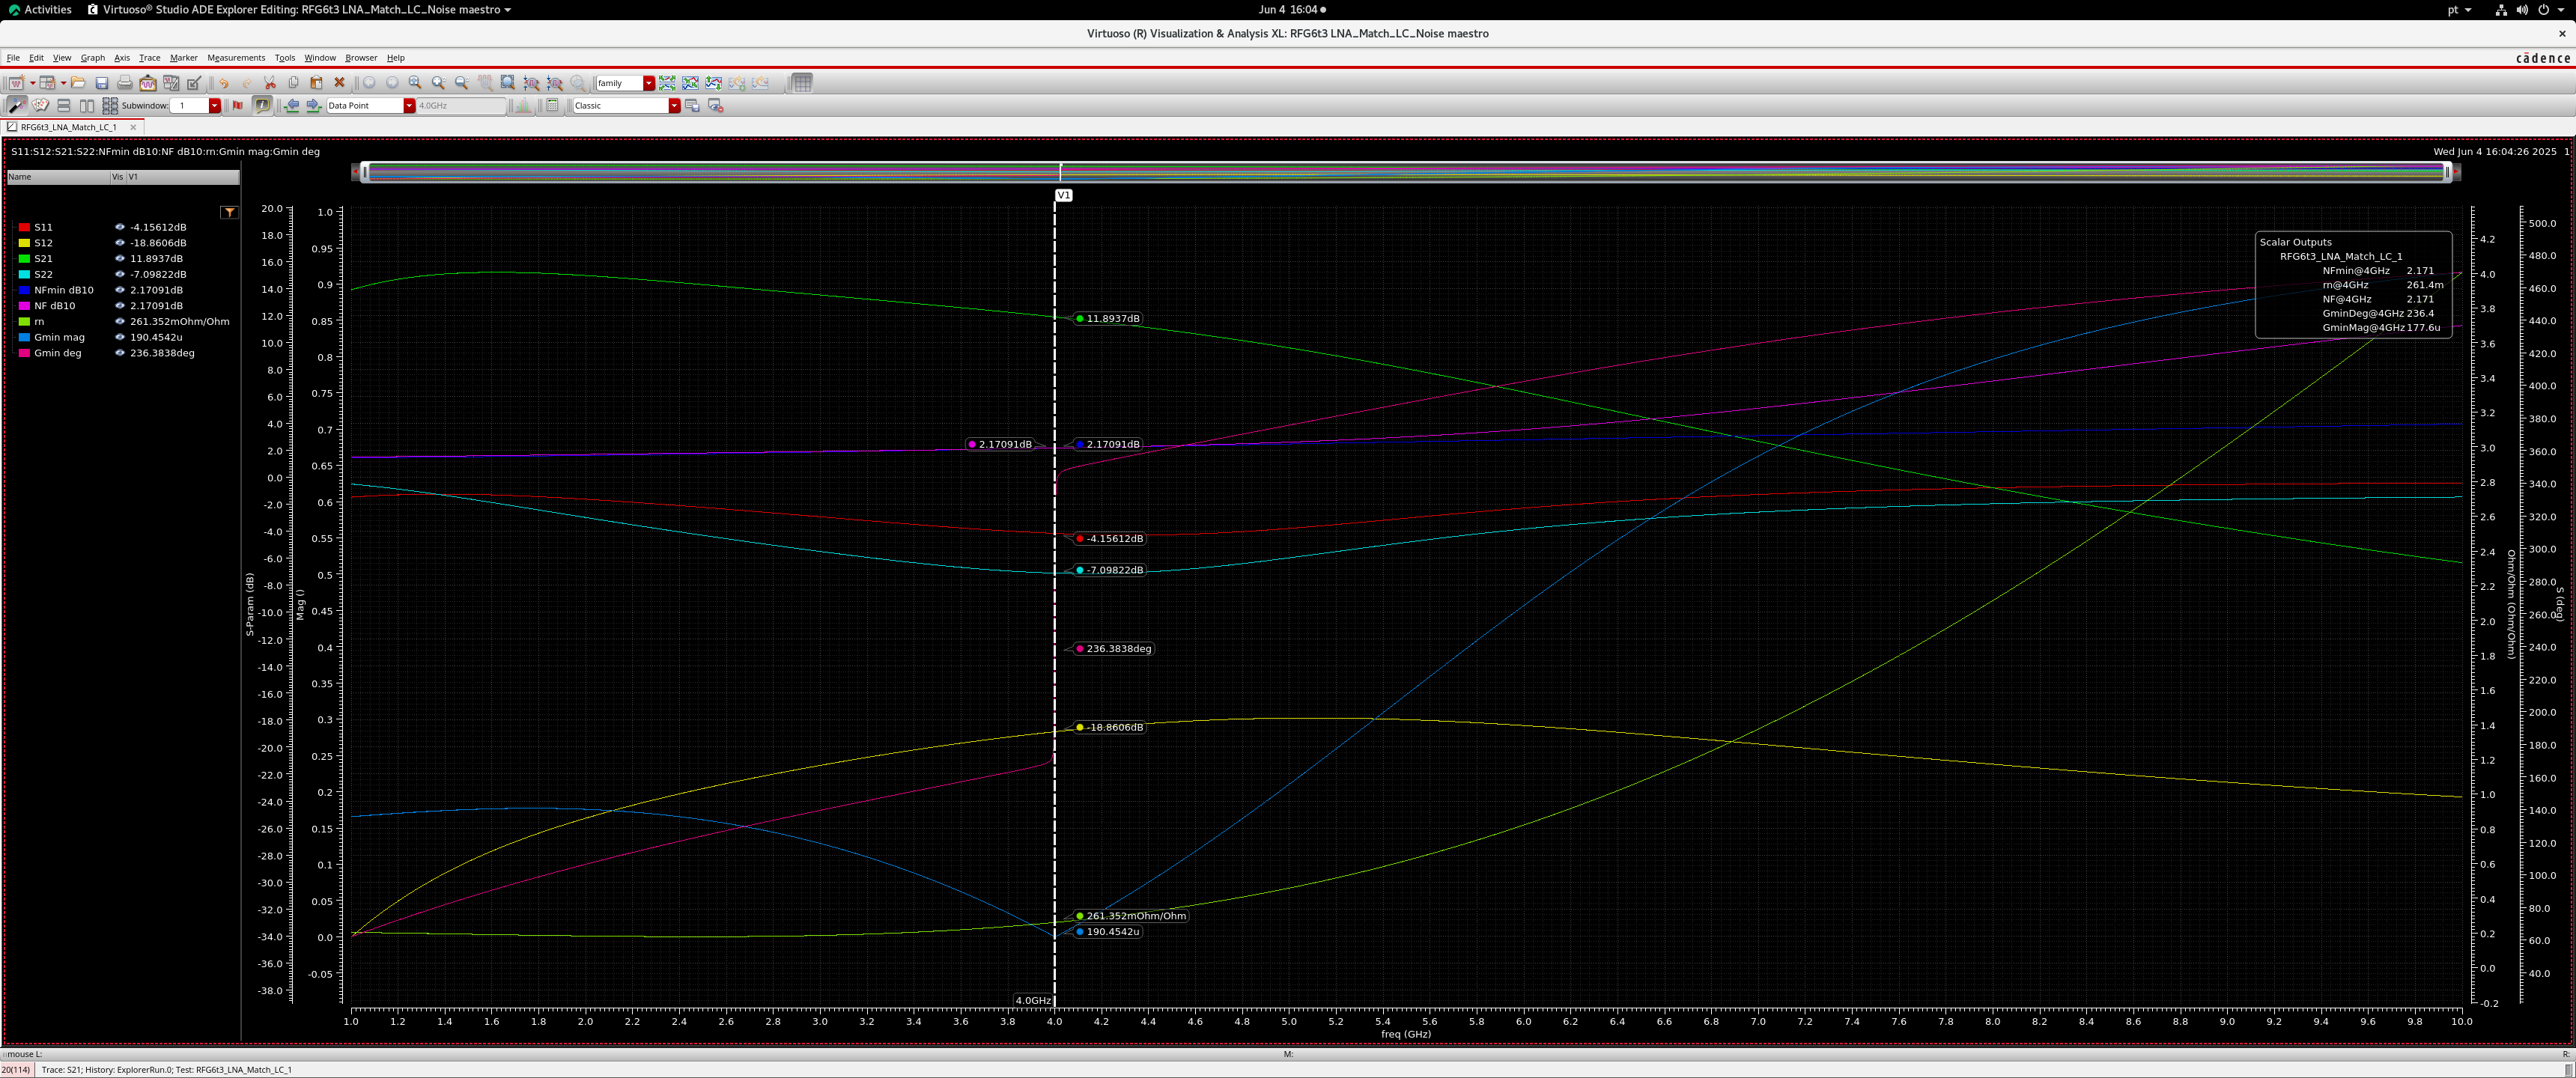
\includegraphics[width=1\textwidth]{Images/CAD-LCmatchNoise.png}
    \caption{Matching networks using lumped circuit elements for minimum noise in Cadence.}
    \label{fig:CadenceNoiseMatchingCircuit}
\end{figure}

In table \ref{tab:NoiseMatchingParameters} the summarized results of the matching networks using lumped circuit elements for minimum noise can be seen.
\begin{table}[H]
    \centering
    \caption{Matching network results for minimum noise in Cadence.}
    \begin{tabularx}{\textwidth}{>{\centering\arraybackslash}X >{\centering\arraybackslash}X}
        \toprule
        \textbf{Parameter} & \textbf{Value} \\
        \midrule
        Theoretical Noise Factor  & $2.17 \si{\decibel}$ \\
        \midrule
        Cadence Noise Factor & $2.17 \si{\decibel}$ \\
        \bottomrule
    \end{tabularx}
    \label{tab:NoiseMatchingParameters}
\end{table}

\subsubsection{Matching networks using transmission lines and stubs}

The matching networks for input and output depicted in Figure \ref{fig:MatchingCircuit-line-noise} were used to perform the simulation and validate the results.

The results of the simulation in Cadence can be seen in Figure \ref{fig:CadenceNoiseMatchingCircuitLine}.
\begin{figure}[H]
    \centering
    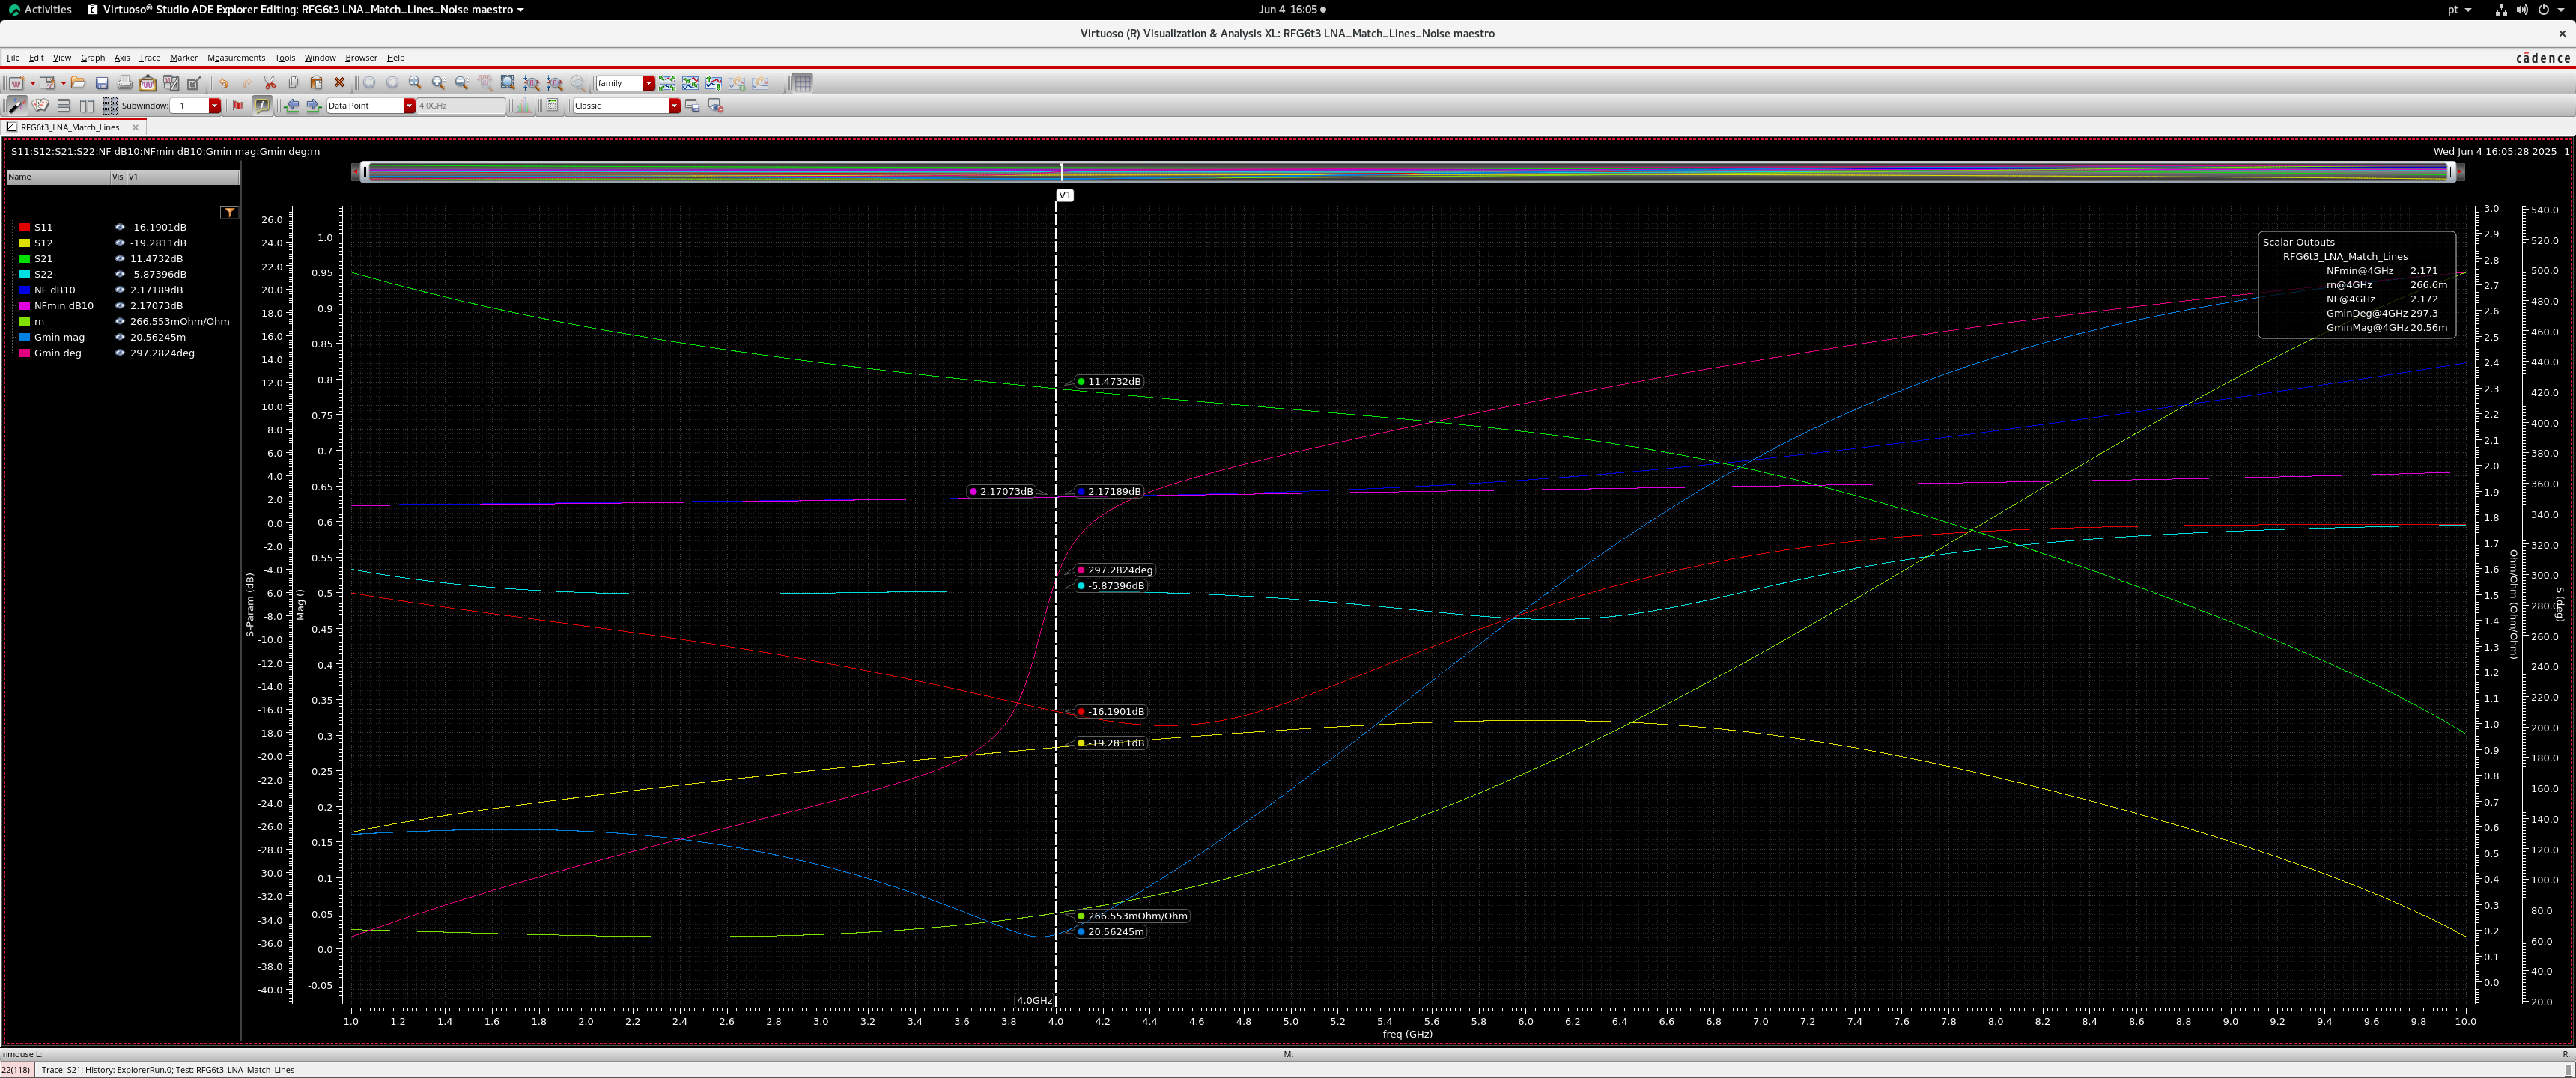
\includegraphics[width=1\textwidth]{Images/CAD-LinesmatchNoise.png}
    \caption{Matching networks using transmission lines and stubs for minimum noise in Cadence.}
    \label{fig:CadenceNoiseMatchingCircuitLine}
\end{figure}

In table \ref{tab:NoiseMatchingParameters} the summarized results of the matching networks using transmission lines and stubs can be seen.
\begin{table}[H]
    \centering
    \caption{Matching network results for minimum noise in Cadence.}
    \begin{tabularx}{\textwidth}{>{\centering\arraybackslash}X >{\centering\arraybackslash}X}
        \toprule
        \textbf{Parameter} & \textbf{Value} \\
        \midrule
        Theoretical Noise Factor  & $2.17 \si{\decibel}$ \\
        \midrule
        Cadence Noise Factor & $2.17 \si{\decibel}$ \\
        \bottomrule
    \end{tabularx}
    \label{tab:NoiseMatchingParameters}
\end{table}

\subsection{Simulation for Noise-Gain Adaptation}

In order to adapt the LNA for minimum noise figure and maximum gain, the matching networks were designed to minimize the noise figure at the desired frequency of $4 GHz$ and maximize the gain at the same frequency, in this section the design matching networks were simulated and validated in Cadence.

\subsubsection{Matching networks using Lumped circuit elements}

The matching networks for input and output depicted in Figure \ref{ffig:MatchingCircuit-gain-noise} were used to perform the simulation and validate the results.

The results of the simulation in Cadence can be seen in Figure \ref{fig:CadenceNoiseGainMatchingCircuit}.
\begin{figure}[H]
    \centering
    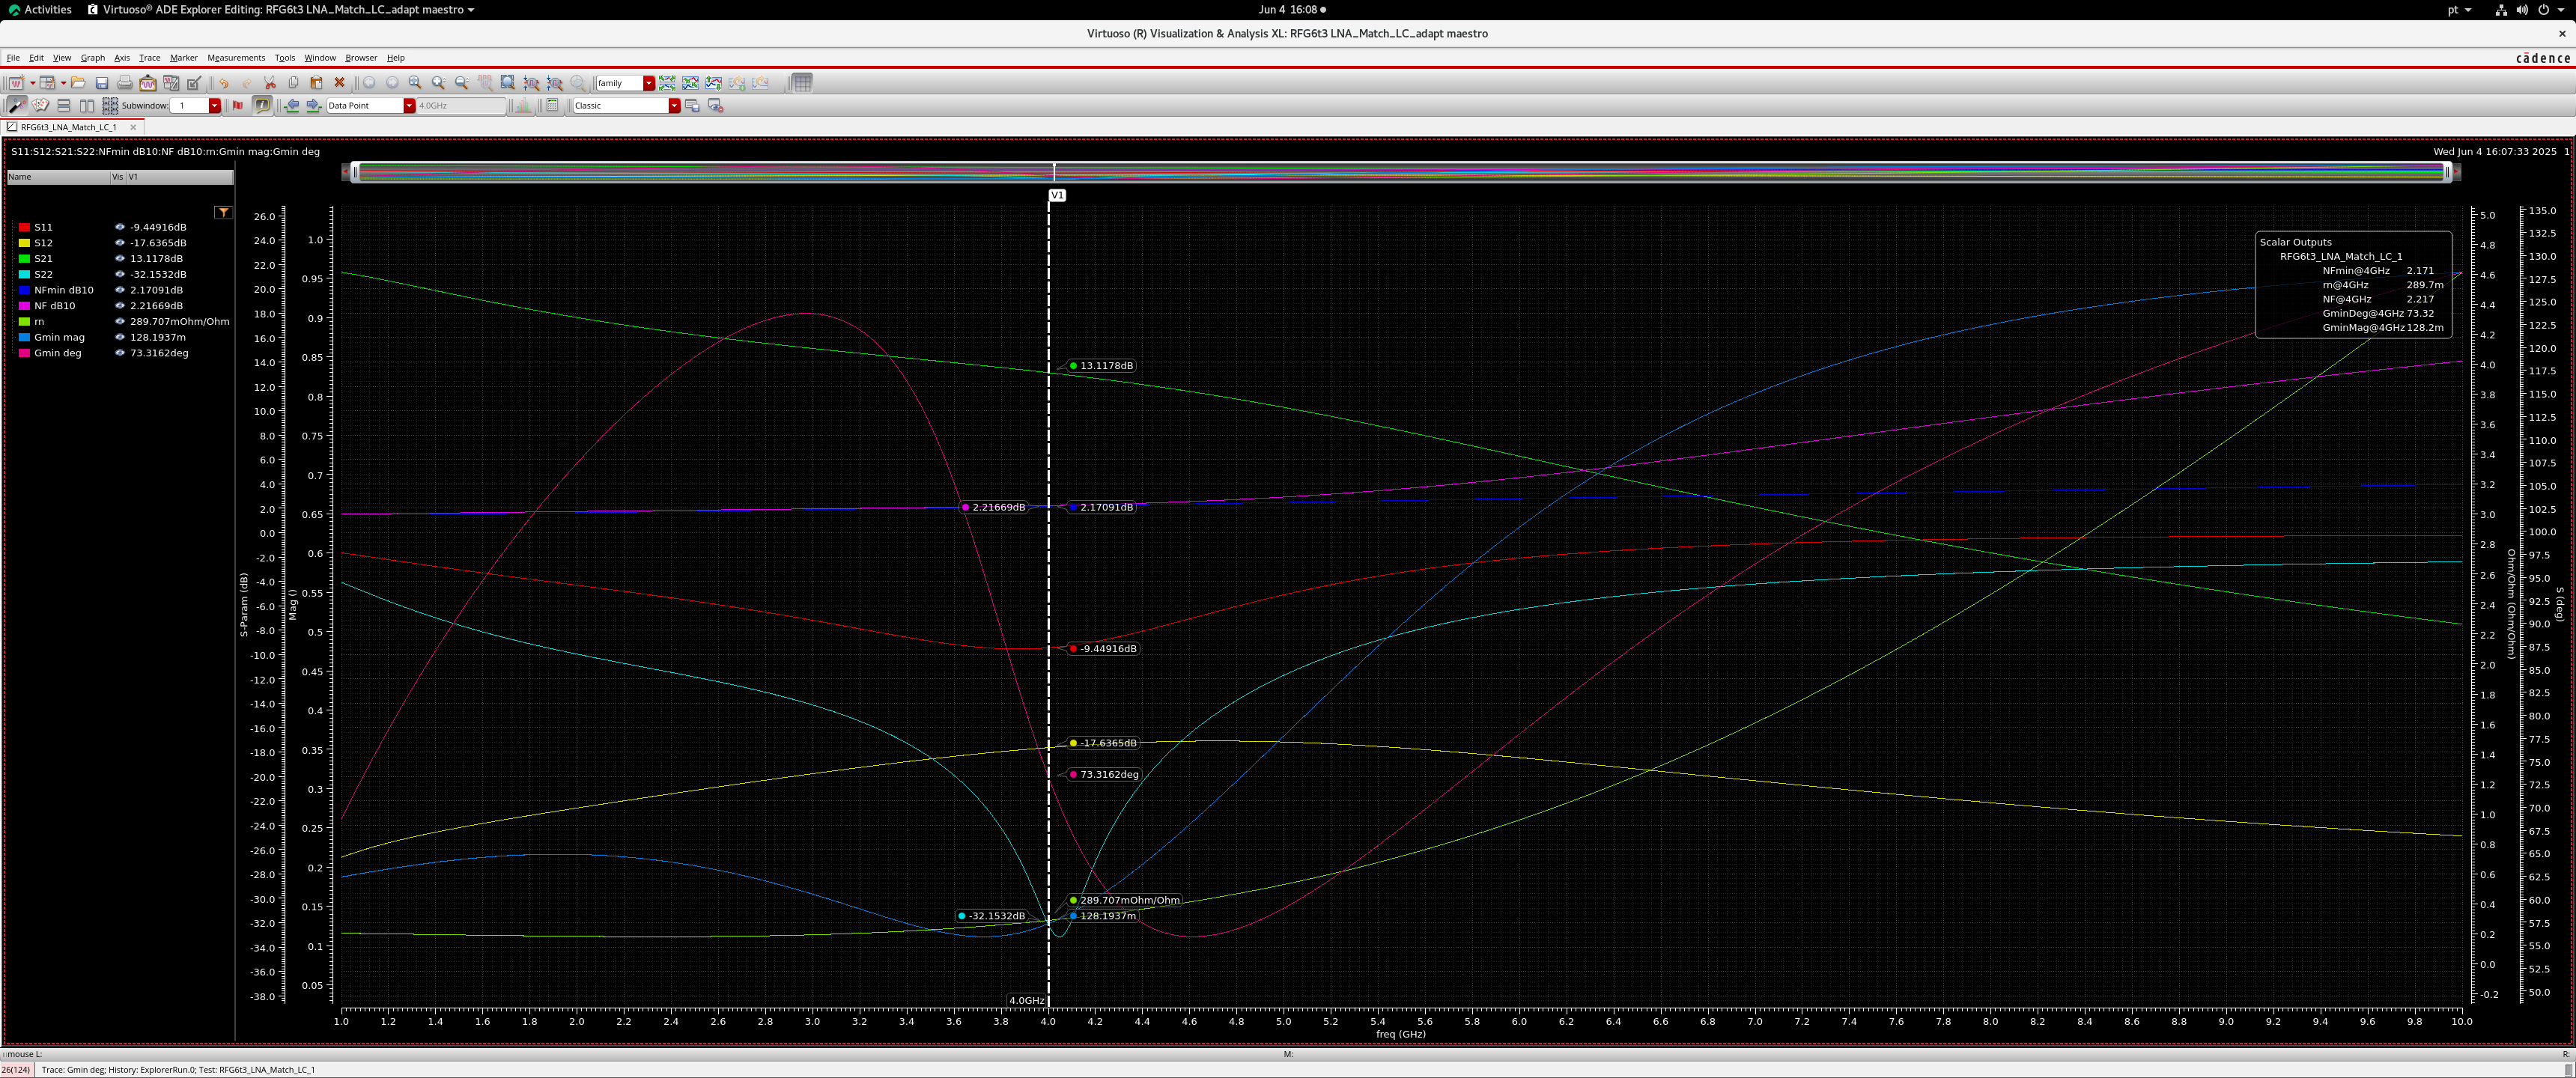
\includegraphics[width=1\textwidth]{Images/CAD_LCmatchNoiseGain.png}
    \caption{Matching networks using lumped circuit elements for minimum noise and maximum gain in Cadence.}
    \label{fig:CadenceNoiseGainMatchingCircuit}
\end{figure}

In table \ref{tab:NoiseGainMatchingParameters} the summarized results of the matching networks using lumped circuit elements for minimum noise and maximum gain can be seen.
\begin{table}[H]
    \centering
    \caption{Lumped elements Matching network results for minimum noise and maximum gain in Cadence.}
    \begin{tabularx}{\textwidth}{>{\centering\arraybackslash}X >{\centering\arraybackslash}X}
        \toprule
        \textbf{Parameter} & \textbf{Value} \\
        \midrule
        Theoretical Noise Factor  & $3 \si{\decibel}$ \\
        \midrule
        Cadence Noise Factor & $2.2 \si{\decibel}$ \\
        \midrule
        Theoretical Gain & $13.22 \si{\decibel}$ \\
        \midrule
        Cadence Gain & $13.11 \si{\decibel}$ \\
        \bottomrule
    \end{tabularx}
    \label{tab:NoiseGainMatchingParameters}
\end{table}

\subsubsection{Matching networks using transmission lines and stubs}

The matching networks for input and output depicted in Figure \ref{fig:MatchingCircuit-line-gain-noise} were used to perform the simulation and validate the results.

The results of the simulation in Cadence can be seen in Figure \ref{fig:CadenceNoiseGainMatchingCircuitLine}.

\begin{figure}[H]
    \centering
    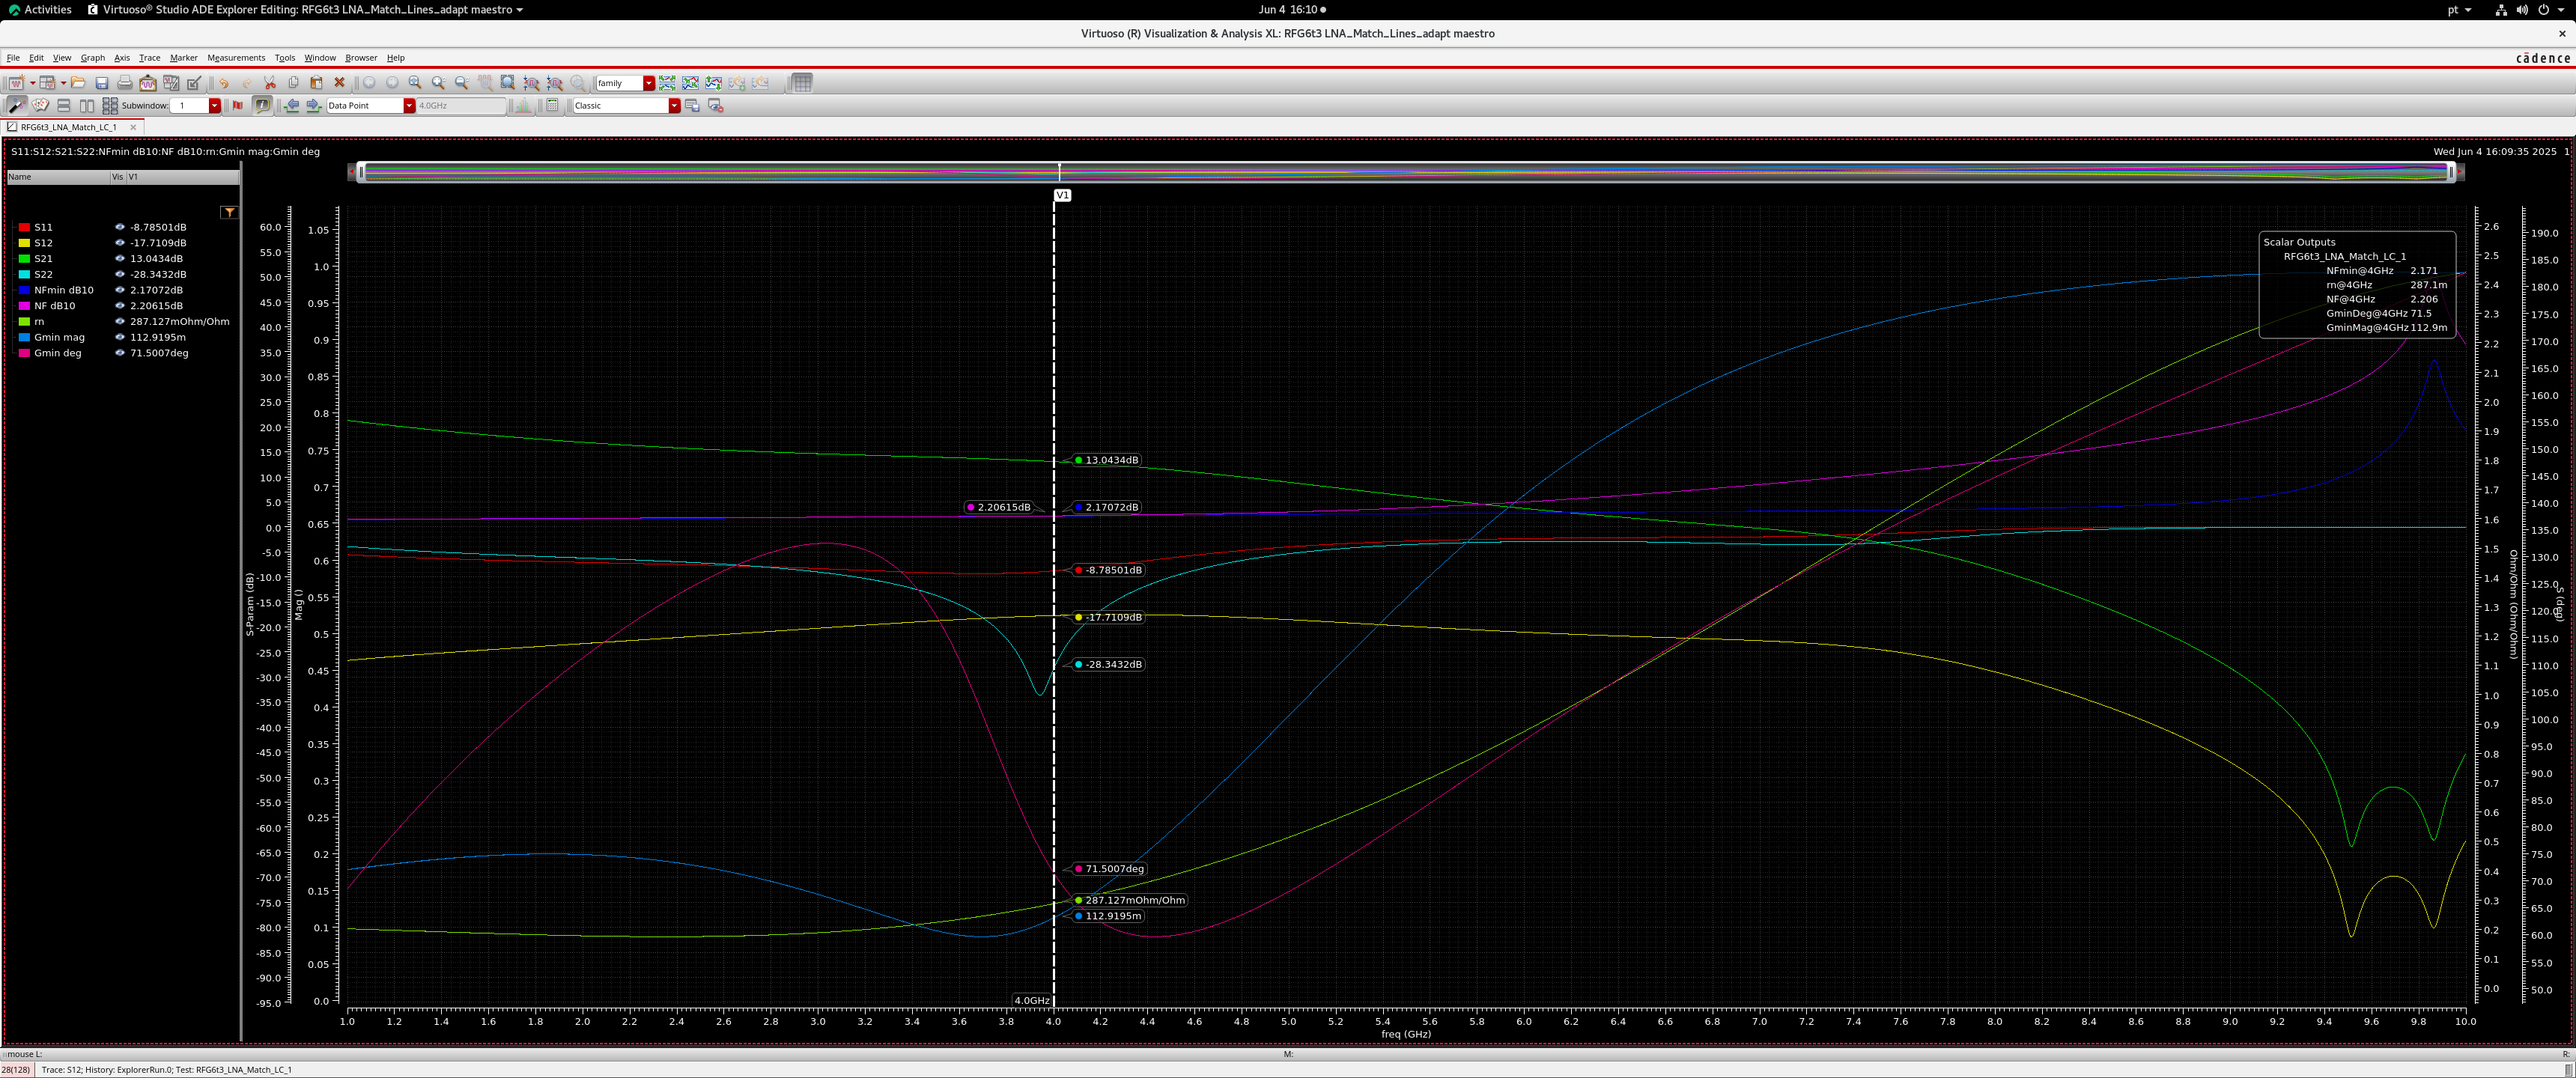
\includegraphics[width=1\textwidth]{Images/CAD-LinesmatchNoiseGain.png}
    \caption{Matching networks using transmission lines and stubs for minimum noise and maximum gain in Cadence.}
    \label{fig:CadenceNoiseGainMatchingCircuitLine}
\end{figure}

In table \ref{tab:NoiseGainMatchingParametersLine} the summarized results of the matching networks using transmission lines and stubs for minimum noise and maximum gain can be seen.
\begin{table}[H]
    \centering
    \caption{Lines and Stubs Matching network results for minimum noise and maximum gain in Cadence.}
    \begin{tabularx}{\textwidth}{>{\centering\arraybackslash}X >{\centering\arraybackslash}X}
        \toprule
        \textbf{Parameter} & \textbf{Value} \\
        \midrule
        Theoretical Noise Factor  & $3 \si{\decibel}$ \\
        \midrule
        Cadence Noise Factor & $2.2 \si{\decibel}$ \\
        \midrule
        Theoretical Gain & $13.22 \si{\decibel}$ \\
        \midrule
        Cadence Gain & $13.04 \si{\decibel}$ \\
        \bottomrule
    \end{tabularx}
    \label{tab:NoiseGainMatchingParametersLine}
\end{table}

The results obtain alongside this section show that the type of matching network used does not affect the noise figure of the circuit or thegain, since both types of matching networks obtained results very close to the theoretical values. The choise of implementation of the matching networks will depend on the application and the available components, since the lumped circuit elements are easier to implement, but the transmission lines and stubs are more suitable for high frequency applications, like this one.